% Options for packages loaded elsewhere
\PassOptionsToPackage{unicode}{hyperref}
\PassOptionsToPackage{hyphens}{url}
\PassOptionsToPackage{dvipsnames,svgnames,x11names}{xcolor}
%
\documentclass[
  letterpaper,
  DIV=11,
  numbers=noendperiod]{scrreprt}

\usepackage{amsmath,amssymb}
\usepackage{iftex}
\ifPDFTeX
  \usepackage[T1]{fontenc}
  \usepackage[utf8]{inputenc}
  \usepackage{textcomp} % provide euro and other symbols
\else % if luatex or xetex
  \usepackage{unicode-math}
  \defaultfontfeatures{Scale=MatchLowercase}
  \defaultfontfeatures[\rmfamily]{Ligatures=TeX,Scale=1}
\fi
\usepackage{lmodern}
\ifPDFTeX\else  
    % xetex/luatex font selection
\fi
% Use upquote if available, for straight quotes in verbatim environments
\IfFileExists{upquote.sty}{\usepackage{upquote}}{}
\IfFileExists{microtype.sty}{% use microtype if available
  \usepackage[]{microtype}
  \UseMicrotypeSet[protrusion]{basicmath} % disable protrusion for tt fonts
}{}
\makeatletter
\@ifundefined{KOMAClassName}{% if non-KOMA class
  \IfFileExists{parskip.sty}{%
    \usepackage{parskip}
  }{% else
    \setlength{\parindent}{0pt}
    \setlength{\parskip}{6pt plus 2pt minus 1pt}}
}{% if KOMA class
  \KOMAoptions{parskip=half}}
\makeatother
\usepackage{xcolor}
\setlength{\emergencystretch}{3em} % prevent overfull lines
\setcounter{secnumdepth}{5}
% Make \paragraph and \subparagraph free-standing
\ifx\paragraph\undefined\else
  \let\oldparagraph\paragraph
  \renewcommand{\paragraph}[1]{\oldparagraph{#1}\mbox{}}
\fi
\ifx\subparagraph\undefined\else
  \let\oldsubparagraph\subparagraph
  \renewcommand{\subparagraph}[1]{\oldsubparagraph{#1}\mbox{}}
\fi


\providecommand{\tightlist}{%
  \setlength{\itemsep}{0pt}\setlength{\parskip}{0pt}}\usepackage{longtable,booktabs,array}
\usepackage{calc} % for calculating minipage widths
% Correct order of tables after \paragraph or \subparagraph
\usepackage{etoolbox}
\makeatletter
\patchcmd\longtable{\par}{\if@noskipsec\mbox{}\fi\par}{}{}
\makeatother
% Allow footnotes in longtable head/foot
\IfFileExists{footnotehyper.sty}{\usepackage{footnotehyper}}{\usepackage{footnote}}
\makesavenoteenv{longtable}
\usepackage{graphicx}
\makeatletter
\def\maxwidth{\ifdim\Gin@nat@width>\linewidth\linewidth\else\Gin@nat@width\fi}
\def\maxheight{\ifdim\Gin@nat@height>\textheight\textheight\else\Gin@nat@height\fi}
\makeatother
% Scale images if necessary, so that they will not overflow the page
% margins by default, and it is still possible to overwrite the defaults
% using explicit options in \includegraphics[width, height, ...]{}
\setkeys{Gin}{width=\maxwidth,height=\maxheight,keepaspectratio}
% Set default figure placement to htbp
\makeatletter
\def\fps@figure{htbp}
\makeatother
\newlength{\cslhangindent}
\setlength{\cslhangindent}{1.5em}
\newlength{\csllabelwidth}
\setlength{\csllabelwidth}{3em}
\newlength{\cslentryspacingunit} % times entry-spacing
\setlength{\cslentryspacingunit}{\parskip}
\newenvironment{CSLReferences}[2] % #1 hanging-ident, #2 entry spacing
 {% don't indent paragraphs
  \setlength{\parindent}{0pt}
  % turn on hanging indent if param 1 is 1
  \ifodd #1
  \let\oldpar\par
  \def\par{\hangindent=\cslhangindent\oldpar}
  \fi
  % set entry spacing
  \setlength{\parskip}{#2\cslentryspacingunit}
 }%
 {}
\usepackage{calc}
\newcommand{\CSLBlock}[1]{#1\hfill\break}
\newcommand{\CSLLeftMargin}[1]{\parbox[t]{\csllabelwidth}{#1}}
\newcommand{\CSLRightInline}[1]{\parbox[t]{\linewidth - \csllabelwidth}{#1}\break}
\newcommand{\CSLIndent}[1]{\hspace{\cslhangindent}#1}

\KOMAoption{captions}{tableheading}
\makeatletter
\@ifpackageloaded{tcolorbox}{}{\usepackage[skins,breakable]{tcolorbox}}
\@ifpackageloaded{fontawesome5}{}{\usepackage{fontawesome5}}
\definecolor{quarto-callout-color}{HTML}{909090}
\definecolor{quarto-callout-note-color}{HTML}{0758E5}
\definecolor{quarto-callout-important-color}{HTML}{CC1914}
\definecolor{quarto-callout-warning-color}{HTML}{EB9113}
\definecolor{quarto-callout-tip-color}{HTML}{00A047}
\definecolor{quarto-callout-caution-color}{HTML}{FC5300}
\definecolor{quarto-callout-color-frame}{HTML}{acacac}
\definecolor{quarto-callout-note-color-frame}{HTML}{4582ec}
\definecolor{quarto-callout-important-color-frame}{HTML}{d9534f}
\definecolor{quarto-callout-warning-color-frame}{HTML}{f0ad4e}
\definecolor{quarto-callout-tip-color-frame}{HTML}{02b875}
\definecolor{quarto-callout-caution-color-frame}{HTML}{fd7e14}
\makeatother
\makeatletter
\makeatother
\makeatletter
\@ifpackageloaded{bookmark}{}{\usepackage{bookmark}}
\makeatother
\makeatletter
\@ifpackageloaded{caption}{}{\usepackage{caption}}
\AtBeginDocument{%
\ifdefined\contentsname
  \renewcommand*\contentsname{Table of contents}
\else
  \newcommand\contentsname{Table of contents}
\fi
\ifdefined\listfigurename
  \renewcommand*\listfigurename{List of Figures}
\else
  \newcommand\listfigurename{List of Figures}
\fi
\ifdefined\listtablename
  \renewcommand*\listtablename{List of Tables}
\else
  \newcommand\listtablename{List of Tables}
\fi
\ifdefined\figurename
  \renewcommand*\figurename{Figure}
\else
  \newcommand\figurename{Figure}
\fi
\ifdefined\tablename
  \renewcommand*\tablename{Table}
\else
  \newcommand\tablename{Table}
\fi
}
\@ifpackageloaded{float}{}{\usepackage{float}}
\floatstyle{ruled}
\@ifundefined{c@chapter}{\newfloat{codelisting}{h}{lop}}{\newfloat{codelisting}{h}{lop}[chapter]}
\floatname{codelisting}{Listing}
\newcommand*\listoflistings{\listof{codelisting}{List of Listings}}
\usepackage{amsthm}
\theoremstyle{definition}
\newtheorem{definition}{Definition}[chapter]
\theoremstyle{definition}
\newtheorem{example}{Example}[chapter]
\theoremstyle{plain}
\newtheorem{theorem}{Theorem}[chapter]
\theoremstyle{remark}
\AtBeginDocument{\renewcommand*{\proofname}{Proof}}
\newtheorem*{remark}{Remark}
\newtheorem*{solution}{Solution}
\makeatother
\makeatletter
\@ifpackageloaded{caption}{}{\usepackage{caption}}
\@ifpackageloaded{subcaption}{}{\usepackage{subcaption}}
\makeatother
\makeatletter
\@ifpackageloaded{tcolorbox}{}{\usepackage[skins,breakable]{tcolorbox}}
\makeatother
\makeatletter
\@ifundefined{shadecolor}{\definecolor{shadecolor}{rgb}{.97, .97, .97}}
\makeatother
\makeatletter
\makeatother
\makeatletter
\makeatother
\ifLuaTeX
  \usepackage{selnolig}  % disable illegal ligatures
\fi
\IfFileExists{bookmark.sty}{\usepackage{bookmark}}{\usepackage{hyperref}}
\IfFileExists{xurl.sty}{\usepackage{xurl}}{} % add URL line breaks if available
\urlstyle{same} % disable monospaced font for URLs
\hypersetup{
  pdftitle={Introduction to Statistical Theory},
  pdfauthor={Eric M Reyes},
  colorlinks=true,
  linkcolor={blue},
  filecolor={Maroon},
  citecolor={Blue},
  urlcolor={Blue},
  pdfcreator={LaTeX via pandoc}}

\title{Introduction to Statistical Theory}
\author{Eric M Reyes}
\date{Updated: 24 August 2023}

\begin{document}
\maketitle
\ifdefined\Shaded\renewenvironment{Shaded}{\begin{tcolorbox}[sharp corners, borderline west={3pt}{0pt}{shadecolor}, enhanced, frame hidden, interior hidden, breakable, boxrule=0pt]}{\end{tcolorbox}}\fi

\renewcommand*\contentsname{Table of contents}
{
\hypersetup{linkcolor=}
\setcounter{tocdepth}{2}
\tableofcontents
}
\bookmarksetup{startatroot}

\hypertarget{preface}{%
\chapter*{Preface}\label{preface}}
\addcontentsline{toc}{chapter}{Preface}

\markboth{Preface}{Preface}

Probability is the field within mathematics that studies and models
random processes. In contrast, Statistics is a discipline separate from
mathematics that uses data to make inference on a population. Like many
other disciplines (e.g., Engineering and the Sciences), while Statistics
is a separate discipline, the theory underlying the discipline relies
heavily on mathematics; for Statistics, probability plays a pivotal
role. The key step in any statistical analysis is characterizing
variability; this is what allows a statistician to make decisions using
data. And, Probability can be used to develop analytical models to
describe that variability. While we do not need proficiency with
probability to be practitioners of statistical methodology, a foundation
in probability models is necessary for developing statistical theory and
helps us see common threads in statistical modeling.

This is not a Probability text; instead, this text acts as a supplement
to an Introductory Statistics course. Our interest is in illustrating
how Probability is applied to support statistical methodology. While we
assume the reader has taken a course in Probability, we review key
results as needed. As this is meant to be used in a Statistics course,
our goals are much different than those of a mathematician. Instead of a
rigorous treatment of Probability theory (axioms, etc.), our focus is on
the application of Probability to Statistics.

Our goal is that this supplement provides a richer experience for those
students entering Statistics with exposure to Probability by leveraging
the connections between the two disciplines.

\bookmarksetup{startatroot}

\hypertarget{sec-fundamentals}{%
\chapter{Essential Probability}\label{sec-fundamentals}}

Probability is a vast field within Mathematics. However, the starting
point for nearly every course in probability is the development of
essential results (or ``probability rules'') based on the Axioms of
Probability --- an agreed upon mathematical framework for describing
probability. While we will not make use of these results directly, it is
helpful to review them as they lurk in the background of many more
useful results.

\hypertarget{probability-of-an-event}{%
\section{Probability of an Event}\label{probability-of-an-event}}

Any process for which the outcome cannot be predicted with certainty is
a random process. The collection of all possible results from this
random process is known as the \textbf{sample space}, and elementary
probability is centered on \textbf{events} (results of interest) within
this sample space.

\begin{definition}[Sample
Space]\protect\hypertarget{def-sample-space}{}\label{def-sample-space}

The sample space for a random process is the collection of all possible
results that we might observe.

\end{definition}

\begin{definition}[Event]\protect\hypertarget{def-event}{}\label{def-event}

A subset of the sample space that is of particular interest.

\end{definition}

The Axioms of Probability are discussed in terms of such events.

\begin{definition}[Axioms of
Probability]\protect\hypertarget{def-axioms}{}\label{def-axioms}

Let \(\mathcal{S}\) be the sample space of a random process. Suppose
that to each event \(A\) within \(\mathcal{S}\), a number denoted by
\(Pr(A)\) is associated with \(A\). If the map \(Pr(\cdot)\) satisfies
the following three axioms, then it is called a \textbf{probability}:

\begin{enumerate}
\def\labelenumi{\arabic{enumi}.}
\tightlist
\item
  \(Pr(A) \geq 0\)
\item
  \(Pr(\mathcal{S}) = 1\)
\item
  If \(\left\{A_1, A_2, \dotsc\right\}\) is a sequence of mutually
  exclusive events in \(\mathcal{S}\), then
\end{enumerate}

\[Pr\left(\bigcup_{i = 1}^{\infty} A_i\right) = \sum_{i = 1}^{\infty} Pr\left(A_i\right).\]

\(Pr(A)\) is said to be the ``probability of \(A\)'' or the
``probability \(A\) occurs.''

\end{definition}

The first axiom states that probabilities cannot be negative. The second
states that probabilities cannot exceed 1 and that something must result
from a random process. The third states that if two events do not
overlap, the probability of the combination of the events is found by
adding up the individual probabilities. This third axiom begins to
develop an idea of probability as an area.
Figure~\ref{fig-fundamentals-venn-diagram} illustrates a hypothetical
sample space \(\mathcal{S}\) with two events \(A\) and \(B\) of
interest. In the figure, the two events share some overlap. Variations
of this graphic are used in probability courses to develop intuition for
several probability rules. What we emphasize is that we are using the
\emph{area} of each event in the figure to represent probability. The
applications of probability we will be studying continue to build on
this idea of probability as an area.

\begin{figure}

{\centering 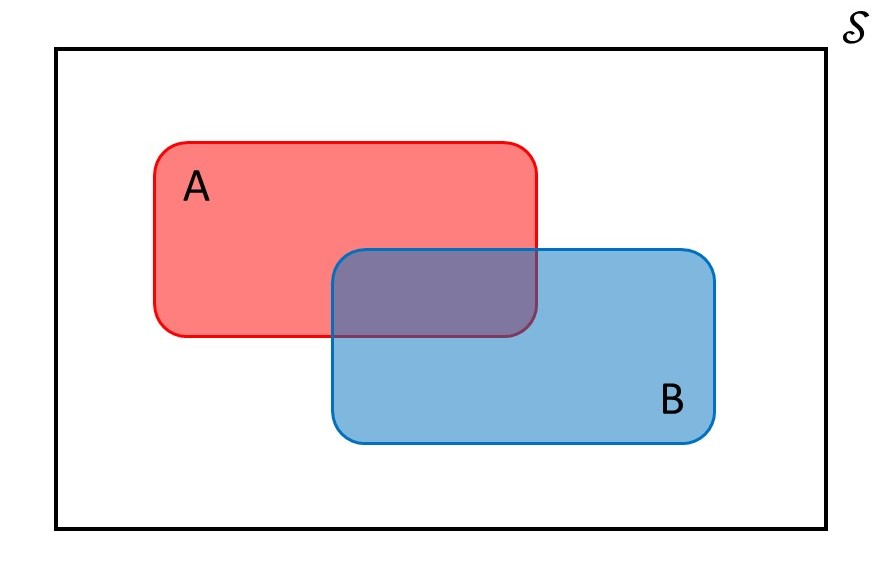
\includegraphics{images/RandomnessVennDiagram.jpg}

}

\caption{\label{fig-fundamentals-venn-diagram}Venn-Diagram illustrating
two events, \(A\) and \(B\), within a sample space \(\mathcal{S}\).}

\end{figure}

\begin{tcolorbox}[enhanced jigsaw, title=\textcolor{quarto-callout-tip-color}{\faLightbulb}\hspace{0.5em}{Big Idea}, colbacktitle=quarto-callout-tip-color!10!white, titlerule=0mm, toptitle=1mm, breakable, bottomtitle=1mm, colframe=quarto-callout-tip-color-frame, opacitybacktitle=0.6, bottomrule=.15mm, arc=.35mm, toprule=.15mm, colback=white, rightrule=.15mm, coltitle=black, leftrule=.75mm, left=2mm, opacityback=0]

Probability represents an area.

\end{tcolorbox}

\hypertarget{essential-results}{%
\section{Essential Results}\label{essential-results}}

While the Axioms of Probability (Definition~\ref{def-axioms}) set the
foundation, we can combine these axioms to form a set of rules which can
be employed to describe a myriad of scenarios. The first rule we review
states that the probability of an event not occurring is equivalent to
subtracting the probability it does occur from 1.

\begin{theorem}[Complement
Rule]\protect\hypertarget{thm-complement-rule}{}\label{thm-complement-rule}

For any event \(A\), the probability of its complement \(A^c\) is given
by

\[Pr\left(A^c\right) = 1 - Pr(A).\]

\end{theorem}

Our interest is not in rigorously developing probability theory; so, we
will offer many results without proof. However, to illustrate the
connection to the axioms, note that the Complement Rule is a result of
the second and third axioms. The second axiom tells us the probability
of the sample space is 1, and the third axiom allows us to consider the
probability of the union of two mutually exclusive events (which an
event and its complement are by definition).

The second rule we consider generalizes the third axiom. The third axiom
considers the union of mutually exclusive events, and the Addition Rule
defines the probability for the union of arbitrary events.

\begin{theorem}[Addition
Rule]\protect\hypertarget{thm-addition-rule}{}\label{thm-addition-rule}

Let \(A\) and \(B\) be arbitrary events, the probability of the union
\(A \cup B\) is given by

\[Pr(A \cup B) = Pr(A) + Pr(B) - Pr(A \cap B)\]

where \(A \cap B\) represents the intersection of the two events.

\end{theorem}

A very helpful technique in mathematical proofs is to ``do nothing.''
This technique will be a recurring theme later in the text and manifests
itself in adding nothing (adding and subtracting the same quantity to an
expression) or multiplying by one (multiplying and dividing an
expression by the same quantity).

\begin{theorem}[Total Probability
Rule]\protect\hypertarget{thm-total-probability-rule}{}\label{thm-total-probability-rule}

Let \(A\) and \(B\) be arbitrary events. Then,

\[Pr(A) = Pr(A \cap B) + Pr\left(A \cap B^c\right).\]

\end{theorem}

Though different than the proof you would likely encounter in a
Probability text, we provide the proof below because it illustrates the
``do nothing'' technique that will be helpful later on.

\begin{proof}

Let \(A\) and \(B\) be arbitrary events. We note that
\(A \cap \mathcal{S}\) is the set \(A\). And, since the intersection of
any set with itself is itself (like multiplying by 1, or ``doing
nothing'' to the set), we have

\[Pr(A) = Pr(A \cap \mathcal{S}).\]

Now, we recognize that an event and its complement together form the
sample space; therefore, we can write

\[Pr(A \cap \mathcal{S}) = Pr\left(A \cap \left(B \cup B^c\right)\right).\]

Using a distributive law from set theory, we write this probability as

\[Pr\left(A \cap \left(B \cup B^c\right)\right) = Pr\left((A \cap B) \cup \left(A \cap B^c\right)\right).\]

We now recognize that the events \((A \cap B)\) and
\(\left(A \cap B^c\right)\) are mutually exclusive. Therefore, applying
the third axiom of probability, we have that

\[Pr\left((A \cap B) \cup \left(A \cap B^c\right)\right) = Pr(A \cap B) + Pr\left(A \cap B^c\right)\]

giving the desired result.

\end{proof}

While there are many other rules that are interesting and useful in
application, the above rules suffice for our purposes.

\hypertarget{interpretation-of-probability}{%
\section{Interpretation of
Probability}\label{interpretation-of-probability}}

Again, most probability courses are focused on the mathematics of
probability; as a result, rarely is the \emph{interpretation} of
probability discussed. In fact, most individuals rarely think about what
they mean by ``the probability an event occurs.'' From a mathematical
perspective, as long as we obey the Axioms of Probability
(Definition~\ref{def-axioms}), we have a probability; its meaning is
irrelevant. But, for practitioners, the interpretation is critical. As
it turns out, there are multiple interpretations of
probability\footnote{See the
  ``\href{https://plato.stanford.edu/archives/win2012/entries/probability-interpret/\#MaiInt}{Interpretations
  of Probability}'' entry in the Stanford Encyclopedia of Philosophy.}.
Two interpretations are of particular interest to us. To illustrate,
consider the following scenario.

\begin{example}[Sugar
Packets]\protect\hypertarget{exm-sugar}{}\label{exm-sugar}

Restaurants can be sources of anxiety for small children. After placing
their order, they must wait (for what seems like an eternity) for that
food to arrive. This is different from their experience at home where
they typically are not brought to the table until it is time to eat.
Parents spend a lot of effort entertaining their children while waiting
for their food to arrive. For parents who do not want to limit screen
time, the following simple game is surprisingly effective:

\begin{quote}
Take one of the sugar packets that is generally available at the table.
Denote the side with the brand name as the ``top side'' and denote the
side with the ingredient list as the ``bottom side.'' The parent then
takes the sugar packet and, hidden from view, tumbles the packet
randomly in their hands. The packet is then placed on the table under
the cover of the parent's hand. The child then declares which side of
the packet is facing up by saying ``top side'' or ``bottom side.''
\end{quote}

This is similar to flipping a coin, but who carries change with them
these days? Consider one round of the above game; suppose the (covered)
packet has been placed on the table and the child says ``top side.'' The
question we ask is then ``what is the probability the child is
correct?''

\end{example}

This simple example illustrates the two commonly applied interpretations
of probability. Most people will say the probability the child is
correct is 0.5. The reasoning is that there are two possibilities (the
top of the sugar packet is face up; or, the bottom of the sugar packet
is face up), and these two possibilities are equally likely (since it
was randomly shuffled before being placed on the table). Therefore, the
probability the child is correct is 0.5. \textbf{This is incorrect from
the lens of this course.} The complication here is that while we are
ignorant of the result (whether the child is correct or not), in
reality, the result has already been determined.

Probability is the study of random processes; in particular, it seeks to
quantify the likelihood that an event \emph{will} occur. Note the use of
the future tense. Once an event has occurred, it does not make sense to
describe the likelihood of the result. Returning to
Example~\ref{exm-sugar}, when a person says that the probability the
child is right is 0.5, what they are really quantifying is not the
likelihood of the child being correct but instead their uncertainty
about that event. This is the ``subjective interpretation'' of
probability.

\begin{definition}[Subjective Interpretation of
Probability]\protect\hypertarget{def-subjective-interpretation}{}\label{def-subjective-interpretation}

In this perspective, the probability of \(A\) describes the individual's
uncertainty about event \(A\).

\end{definition}

Because the subjective interpretation is quantifying an individual's
uncertainty, and since each individual may have different
beliefs/information/expertise about the random process, each individual
observing the same process may have a different probability. For
example, consider asking the question ``what is the probability that
Netflix saves the latest television series dropped by ABC?'' A casual
viewer may have little information regarding this process and will rely
solely on what they perceive the popularity of the show was among its
fan base and news reports they have read online; they may quantify their
uncertainty by saying the probability is 0.65. In contrast, an executive
at Netflix who is deeply familiar with both the show, its fan base, its
ratings in various markets, the interest of leadership to invest in a
new series, and the amount they stand to earn by acquiring the property
has a different set of knowledge; they may quantify their uncertainty by
saying the probability is 0.05. The same process is viewed differently
by different observers, leading to different answers.

Statisticians who adhere to the subjective interpretation of probability
are known as Bayesians. While this interpretation leads to a very
interesting development of statistical theory (we encourage everyone to
take a course in Bayesian Data Analysis), this is not the predominant
interpretation. Classically, statistical theory was developed under the
frequentist interpretation, and statisticians who adhere to this
perspective are known as Frequentists.

\begin{definition}[Frequentist Interpretation of
Probability]\protect\hypertarget{def-frequentist-interpretation}{}\label{def-frequentist-interpretation}

In this perspective, the probability of \(A\) describes the long-run
behavior of the event. Specifically, consider repeating the random
process \(m\) times, and let \(f(A)\) represent the number of times the
event \(A\) occurs out of those \(m\) replications. Then,

\[Pr(A) = \lim_{m \rightarrow \infty} \frac{f(A)}{m}.\]

\end{definition}

The frequentist interpretation requires repeating a process infinitely
often. When characterizing the probability of an event, the frequentist
perspective leans on the future-oriented nature of probability. When we
are characterizing the probability an event \emph{will} occur
(future-oriented), we are really thinking about repeating that process
infinitely often and determining what fraction of the time the event
occurs; we then apply that to the specific process we are about to
observe. Of course, this does not always make sense in practice. For
example, asking ``what is the probability that Candidate A will win the
upcoming election'' is a one time event. The election cannot be held
infinitely often; it will only be held once. In these cases, the
frequentist interpretation still \emph{imagines} infinitely many of
these elections. For those who are fans of science fiction, you can
think of the frequentist perspective as finding the limit over the
infinitely many instances in the multiverse (the proportion of times
Candidate A wins the election across all instances of the election in
the multiverse). The frequentist perspective is ``objective'' in the
sense that it does not incorporate the observer's personal
beliefs/information/expertise regarding the process.

Returning to Example~\ref{exm-sugar}, since the result has already
occurred, probability does not make sense. Further, since the
frequentist perspective does not quantify our uncertainty about the
result (as the subjective perspective does), we are left saying that the
probability that the child is correct is either 1 (they are correct) or
0 (they are not correct). Admittedly, this is unsatisfying, but we must
remember that the frequentist interpretation is not interested in
quantifying our uncertainty; it is only interested in the proportion of
times the result will occur, and since the result is in the past, it
either has occurred (proportion of 1) or it has not (proportion of 0).

This may seem like arguing over semantics, and admittedly, the
importance of this discussion is not yet clear. But, we will see that
how probability is interpreted impacts how we interpret the results of
our statistical analyses.

\begin{tcolorbox}[enhanced jigsaw, title=\textcolor{quarto-callout-tip-color}{\faLightbulb}\hspace{0.5em}{Big Idea}, colbacktitle=quarto-callout-tip-color!10!white, titlerule=0mm, toptitle=1mm, breakable, bottomtitle=1mm, colframe=quarto-callout-tip-color-frame, opacitybacktitle=0.6, bottomrule=.15mm, arc=.35mm, toprule=.15mm, colback=white, rightrule=.15mm, coltitle=black, leftrule=.75mm, left=2mm, opacityback=0]

The frequentist interpretation of probability does not quantify our
uncertainty about an event; it quantifies the likelihood of an event in
repeated observation.

\end{tcolorbox}

\bookmarksetup{startatroot}

\hypertarget{sec-randomvariables}{%
\chapter{Random Variables and Distributions}\label{sec-randomvariables}}

In Chapter~\ref{sec-fundamentals}, we discussed the probability of an
``event.'' For statisticians, the events of interests center on
measurements, or functions of those measurements, that we plan to take.
In this chapter, we begin to connect probability to data analysis. Our
goal is to reexamine concepts introduced in a probability course,
relating them to their data-centric analogues.

\hypertarget{random-variables}{%
\section{Random Variables}\label{random-variables}}

Consider collecting data; before the data is collected, we cannot
predict with certainty what we will observe. Therefore, we can think of
each observation as the result of a random process. These observations
are recorded as variables in our dataset. In probability, a
\textbf{random variable} is used to represent a measurement that results
from a random process.

\begin{definition}[Random
Variable]\protect\hypertarget{def-random-variable}{}\label{def-random-variable}

Let \(\mathcal{S}\) be the sample space corresponding to a random
process; a random variable \(X\) is a function mapping elements of the
sample space to the real line.

Random variables represent a measurement that will be collected during
the course of a study. Random variables are typically represented by a
capital letter.

\end{definition}

While for our purposes, it suffices to think of a random variable as a
measurement, mathematically, it is a \emph{function}. The image (or
range) of this function is used to broadly classify random variables as
\textbf{continuous} or \textbf{discrete}; we refer to this image as the
\textbf{support} of the random variable.

\begin{definition}[Support]\protect\hypertarget{def-support}{}\label{def-support}

The support of a random variable is the set of all possible values the
random variable can take.

\end{definition}

\begin{definition}[Continuous and Discrete Random
Variable]\protect\hypertarget{def-rvtypes}{}\label{def-rvtypes}

The random variable \(X\) is said to be a discrete random variable if
its corresponding support is countable. The random variable \(X\) is
said to be a continuous random variable if the corresponding support is
uncountable (such as an interval or a union of intervals on the real
line).

\end{definition}

Discrete random variables are analogous to categorical (or qualitative)
variables in data analysis; that is, discrete random variables are used
to model the result of a random process which categorizes each unit of
observation into a group. Continuous random variables are analogous to
numeric (or quantitative) variables in data analysis; continuous random
variables are used to model the result of a random process which
produces a number for which arithmetic makes sense.

\begin{tcolorbox}[enhanced jigsaw, title=\textcolor{quarto-callout-warning-color}{\faExclamationTriangle}\hspace{0.5em}{Warning}, colbacktitle=quarto-callout-warning-color!10!white, titlerule=0mm, toptitle=1mm, breakable, bottomtitle=1mm, colframe=quarto-callout-warning-color-frame, opacitybacktitle=0.6, bottomrule=.15mm, arc=.35mm, toprule=.15mm, colback=white, rightrule=.15mm, coltitle=black, leftrule=.75mm, left=2mm, opacityback=0]

Whether we use a continuous or discrete random variable to represent a
measurement is not always obvious. Suppose we consider recording the age
of a student selected from a class at a university that typically
enrolls ``traditional'' students (those coming directly from high
school). Let the random variable \(X\) denote the age of the student.

If we record the student's age in years since birth, \(X\) can take on
only a finite number of values (most likely
\(\{18, 19, 20, 21, 22, 23\}\)), making it a discrete random variable.
However, if we record the student's age as the number of seconds since
birth, we might well consider the support of \(X\) to be a rather large
interval, leading to a continuous random variable.

\end{tcolorbox}

The goal of statistics is to use a sample to say something about the
underlying population. Consider taking a sample of size \(n\) and
measuring a single variable on each unit of observation. Then, we might
represent the measurements we will obtain (note the use of the future
tense) as \(X_1, X_2, \dots, X_n\). While the majority of probability
courses focus on a single, or maybe two, random variables, note that
collecting data on a sample requires that we deal with at least \(n\)
random variables (one measurement for each of the observations in our
sample).

\hypertarget{characterizing-a-distribution}{%
\section{Characterizing a
Distribution}\label{characterizing-a-distribution}}

Again, the goal of statistics is to use a sample to say something about
the underlying population. Consider the following research objective:

\begin{quote}
Estimate the cost (in US dollars) of a diamond for sale in the United
States.
\end{quote}

For this research objective, our population of interest is all diamonds
for sale in the United States. We would not expect every diamond for
sale to have the same price; variability is inherent in any process. As
a result, the sale price of diamonds has a distribution across this
population. This is our primary use of probability theory in a
statistical analysis --- to model distributions.

Consider taking a sample of size 1 from the population; let \(Y\)
represent the cost of the diamond that is selected. Since we have not
yet observed the cost of this diamond, \(Y\) is a random variable. And,
since this diamond is sampled from the population of interest, the
support of \(Y\) is determined by the cost of diamonds in the United
States. Further, the likelihood that \(Y\) falls within any interval is
determined by the distribution of the cost across the population. That
is, the distribution of \(Y\) is the distribution of the population.

\begin{tcolorbox}[enhanced jigsaw, title=\textcolor{quarto-callout-tip-color}{\faLightbulb}\hspace{0.5em}{Big Idea}, colbacktitle=quarto-callout-tip-color!10!white, titlerule=0mm, toptitle=1mm, breakable, bottomtitle=1mm, colframe=quarto-callout-tip-color-frame, opacitybacktitle=0.6, bottomrule=.15mm, arc=.35mm, toprule=.15mm, colback=white, rightrule=.15mm, coltitle=black, leftrule=.75mm, left=2mm, opacityback=0]

If a random variable \(X\) represents a measurement for a single
observation from a population, the distribution of the random variable
corresponds to the distribution of the variable across the population.

\end{tcolorbox}

A key realization in statistical analysis is that we will never fully
observe the distribution of the population; however, we can posit a
model for this distribution. In probability, the most common way to
characterize the distribution of a random variable is through its
density function.

\begin{definition}[Density
Function]\protect\hypertarget{def-density-function}{}\label{def-density-function}

A density function \(f\) relates the values in the support of a random
variable with the probability of observing those values.

Let \(X\) be a continuous random variable, then its density function
\(f\) is the function such that

\[Pr(a \leq X \leq b) = \int_a^b f(x) dx\]

for any real numbers \(a\) and \(b\) in the support.

Let \(X\) be a discrete random variable, then its density function \(f\)
is the function such that

\[Pr(X = u) = f(u)\]

for any real number \(u\) in the support.

\end{definition}

\begin{tcolorbox}[enhanced jigsaw, title=\textcolor{quarto-callout-note-color}{\faInfo}\hspace{0.5em}{Properties of a Density Function}, colbacktitle=quarto-callout-note-color!10!white, titlerule=0mm, toptitle=1mm, breakable, bottomtitle=1mm, colframe=quarto-callout-note-color-frame, opacitybacktitle=0.6, bottomrule=.15mm, arc=.35mm, toprule=.15mm, colback=white, rightrule=.15mm, coltitle=black, leftrule=.75mm, left=2mm, opacityback=0]

Let \(X\) be a random variable with density function \(f\) defined over
support \(\mathcal{S}\). Then,

\begin{enumerate}
\def\labelenumi{\arabic{enumi}.}
\tightlist
\item
  \(f(x) \geq 0\) for all \(x \in \mathcal{S}\). That is, the density is
  non-negative for all values in the support.
\item
  If \(X\) is a continuous random variable, then
  \(\int_{\mathcal{S}} f(x) dx = 1\); similarly, if \(X\) is a discrete
  random variable, then \(\sum_{\mathcal{S}} f(x) = 1\). That is, \(X\)
  must take a value in its support; so, \(Pr(X \in \mathcal{S}) = 1\),
  similar to the second Axiom of Probability
  (Definition~\ref{def-axioms}).
\item
  \(f(x) = 0\) for all values of \(x \notin \mathcal{S}\). The density
  takes the value of 0 for all values outside the support.
\end{enumerate}

\end{tcolorbox}

\begin{tcolorbox}[enhanced jigsaw, title=\textcolor{quarto-callout-note-color}{\faInfo}\hspace{0.5em}{Note}, colbacktitle=quarto-callout-note-color!10!white, titlerule=0mm, toptitle=1mm, breakable, bottomtitle=1mm, colframe=quarto-callout-note-color-frame, opacitybacktitle=0.6, bottomrule=.15mm, arc=.35mm, toprule=.15mm, colback=white, rightrule=.15mm, coltitle=black, leftrule=.75mm, left=2mm, opacityback=0]

In a probability course, there is often a distinction made between
probability ``density'' functions (used for continuous random variables)
and probability ``mass'' functions (used for discrete random variables).
We do not make this distinction and instead rely on the context to
determine whether we are dealing with a continuous or discrete random
variable. Throughout, we will note when the operations differ between
these two types of variables. Measure theory provides a unifying
framework to these issues.

\end{tcolorbox}

With few exceptions, we will be working with continuous random
variables. As a result, the density function is a smooth function over
some region, and the actual value of the function is not interpretable;
instead, we get at a probability by considering the area under the
curve. Again, drawing connections to data analysis, we can think of a
density function as a mathematical formula representing a smooth
histogram. The area under the curve for any region gives the proportion
of the population which has a value in that region. That is, we get the
probability that a random variable will be in an interval by integrating
the density function over that interval.

Figure Figure~\ref{fig-randomvariables-density} illustrates this idea;
we have data from a sample of diamonds from the population of interest.
The sample is summarized with a histogram; we have overlayed a posited
density (with the corresponding mathematical function that describes
this density) for the population. The sample (summarized with the
histogram) is approximating the population (modeled using the density
function).

\begin{figure}

{\centering 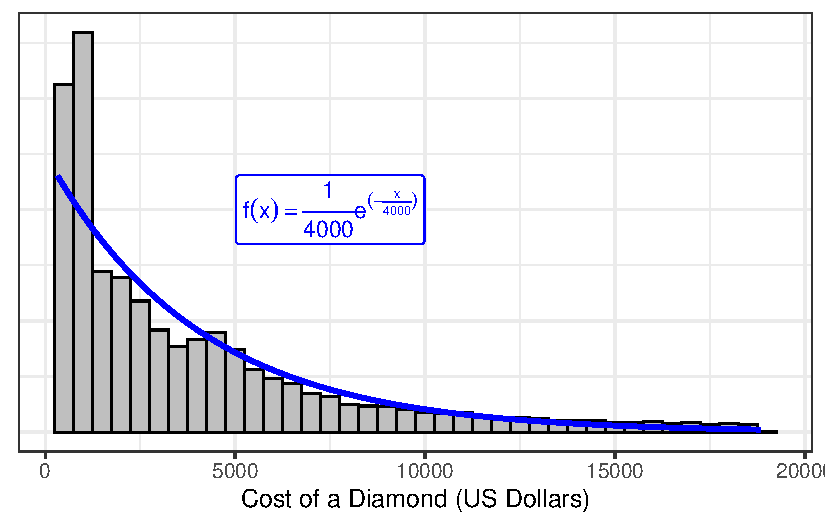
\includegraphics[width=0.8\textwidth,height=\textheight]{./images/fig-randomvariables-density-1.pdf}

}

\caption{\label{fig-randomvariables-density}Illustration of a density
function representing the posited distribution of the population
alongside a histogram summarizing the cost of diamonds using a sample of
53940 diamonds.}

\end{figure}

You may recognize the particular form of the density function in
Figure~\ref{fig-randomvariables-density}. The general form is

\[f(x) = \frac{1}{\sigma} e^{-x / \sigma} \qquad \text{for } x > 0\]

where \(\sigma\) is the \emph{scale} parameter that defines the
distribution (set at 4000 in Figure~\ref{fig-randomvariables-density}).
This is known as the Exponential distribution with scale parameter
\(\sigma\). This illuminates another connection between probability and
statistics.

Note that our research objective describe above is an ill-posed question
as stated. The answer is ``it depends'' since each individual diamond in
the population has a different value. Well-posed questions in statistics
are centered on an appropriately chosen \textbf{parameter}.

\begin{definition}[Parameter]\protect\hypertarget{def-parameter}{}\label{def-parameter}

Numeric quantity which summarizes the distribution of a variable within
the \emph{population} of interest. Generally denoted by Greek letters in
statistical formulas.

\end{definition}

In probability, the parameters are values that are tuned or set within a
problem; we then work forward to compute the probability of an event of
interest. In practice, however, when we posit a functional form for a
density function to describe the distribution of the population, the
parameters are unknown. We plan to use the data to estimate or
characterize the parameter; but, the parameter itself will remain
unknown. In both cases, however, the parameter is a \emph{fixed
quantity}, even if we are ignorant of that value.

\begin{tcolorbox}[enhanced jigsaw, title=\textcolor{quarto-callout-tip-color}{\faLightbulb}\hspace{0.5em}{Big Idea}, colbacktitle=quarto-callout-tip-color!10!white, titlerule=0mm, toptitle=1mm, breakable, bottomtitle=1mm, colframe=quarto-callout-tip-color-frame, opacitybacktitle=0.6, bottomrule=.15mm, arc=.35mm, toprule=.15mm, colback=white, rightrule=.15mm, coltitle=black, leftrule=.75mm, left=2mm, opacityback=0]

When a probability model is specified for a population, it is generally
specified up to some unknown parameter(s). Making inference on the
unknown parameter(s) therefore characterizes the entire distribution.

\end{tcolorbox}

\hypertarget{common-parameters}{%
\subsection{Common Parameters}\label{common-parameters}}

Most scientific questions are focused on the location or spread of a
distribution. For example, we are interested in estimating the average
cost of a diamond sold in the United States. Introductory statistics
introduces summaries of location and spread within the sample (e.g.,
sample mean for location and sample variance for spread). Analogous
summaries exist for density functions. As stated above, parameters are
unknown constants that govern the form of the density function. Because
they govern the form of the density, the parameters are also related to
those summarizing the location or spread of the distribution.

\begin{definition}[Expected Value
(Mean)]\protect\hypertarget{def-mean}{}\label{def-mean}

Let \(X\) be a random variable with density function \(f\) defined over
the support \(\mathcal{S}\). The expected value of a random variable,
also called the mean and denoted \(E(X)\), is given by

\[E(X) = \int_{\mathcal{S}} x f(x) dx\]

for continuous random variables and

\[E(X) = \sum_{\mathcal{S}} x f(x)\]

for discrete random variables.

\end{definition}

Notice the similarity between the form of the sample mean and the
population mean. A sample mean takes the sum of each value in the
sample, weighting each value by \(1/n\) (where \(n\) is the sample
size). Without information about the underlying population, the sample
must treat each value observed as equally likely; values become more
likely if they appear multiple times. In the population, however, when
the form of \(f\) is known, the density provides information about the
likelihood of each value giving us a better weight than \(1/n\). That
is, the population mean is a sum of the values in the support, weighting
each value by the corresponding value of the density function.

\begin{definition}[Variance]\protect\hypertarget{def-variance}{}\label{def-variance}

Let \(X\) be a random variable with density function \(f\) defined over
the support \(\mathcal{S}\). The variance of a random variable, denoted
\(Var(X)\), is given by

\[Var(X) = E\left[X - E(X)\right]^2 = E\left(X^2\right) - E^2(X).\]

If we let \(\mu = E(X)\), then this is equivalent to

\[\int_{\mathcal{S}} (x - \mu)^2 f(x) dx\]

for continuous random variables and

\[\sum_{\mathcal{S}} (x - \mu)^2 f(x)\]

for discrete random variables.

\end{definition}

\begin{tcolorbox}[enhanced jigsaw, title=\textcolor{quarto-callout-warning-color}{\faExclamationTriangle}\hspace{0.5em}{Warning}, colbacktitle=quarto-callout-warning-color!10!white, titlerule=0mm, toptitle=1mm, breakable, bottomtitle=1mm, colframe=quarto-callout-warning-color-frame, opacitybacktitle=0.6, bottomrule=.15mm, arc=.35mm, toprule=.15mm, colback=white, rightrule=.15mm, coltitle=black, leftrule=.75mm, left=2mm, opacityback=0]

Pay careful attention to the notation. \(E^2(X)\) represents the square
of the expected value; that is,

\[E^2(X) = \left[E(X)\right]^2.\]

However, \(E(X)^2\) represents the expected value of the square of
\(X\); that is,

\[E(X)^2 = E\left(X^2\right).\]

\end{tcolorbox}

The variance provides a measure of spread; in particular, it is
capturing distance from the mean. Notice that the form of the variance
involves taking the expectation of a squared term; in general, we will
need to consider expectations of functions.

\begin{definition}[Expectation of a
Function]\protect\hypertarget{def-expectation}{}\label{def-expectation}

Let \(X\) be a random variable with density function \(f\) over the
support \(\mathcal{S}\), and let \(g\) be a real-valued function. Then,

\[E\left[g(X)\right] = \int_{\mathcal{S}} g(x) f(x) dx\]

for continuous random variables and

\[E\left[g(X)\right] = \sum_{\mathcal{S}} g(x) f(x)\]

for discrete random variables.

\end{definition}

A result of Definition~\ref{def-expectation} is the following, very
useful theorem, which states that expectations are linear operators.

\begin{theorem}[Expectation of a Linear
Combination]\protect\hypertarget{thm-expectation}{}\label{thm-expectation}

Let \(X\) be a random variable, and let \(a_1, a_2, \dotsc, a_m\) be
real-valued constants and \(g_1, g_2, \dotsc, g_m\) be real-valued
functions; then,

\[E\left[\sum_{i=1}^{m} a_i g_i(X)\right] = \sum_{i=1}^{m} a_i E\left[g_i(X)\right].\]

\end{theorem}

The mean and variance play an important role in characterizing a
distribution, especially within statistical theory (as we will see in
future chapters). However, there is another set of parameters which are
important.

\begin{definition}[Percentile]\protect\hypertarget{def-percentile}{}\label{def-percentile}

Let \(X\) be a random variable with density function \(f\). The \(100k\)
percentile is the value \(q\) such that

\[Pr(X \leq q) = k.\]

\end{definition}

\begin{example}[Parameters of Exponential
Distribution]\protect\hypertarget{exm-parameters}{}\label{exm-parameters}

Let \(X\) be an Exponential distribution with scale parameter
\(\sigma\); that is, the density function \(f\) is given by

\[f(x) = \frac{1}{\sigma} e^{-x/\sigma} \qquad x > 0\]

where \(\sigma > 0.\) Compute the mean, variance, and median of this
distribution, as a function of the unknown scale parameter.

\end{example}

The solution to this problem is particularly important as it illustrates
a very useful technique when working with known distributions in
statistical theory.

\begin{solution}

We note that the function

\[g(y) = \frac{1}{\beta^{\alpha} \Gamma(\alpha)} y^{\alpha - 1} e^{-y/\beta}\]

is a valid density function over the positive real line provided that
\(\alpha,\beta > 0\); in particular, this is known as a Gamma
distribution. Since \(g\) is a valid density function, then we know that

\[\int_{0}^{\infty} g(y) dy = 1\]

for all values of \(\alpha,\beta > 0\).

Now, let \(X\) be an Exponential random random variable with scale
parameter \(\sigma\). Then, the expected value of \(X\) is given by

\[
\begin{aligned}
  E(X)
    &= \int_{0}^{\infty} x \frac{1}{\sigma} e^{-x/\sigma} dx \\
    &= \int_{0}^{\infty} \frac{1}{\sigma} x^{2-1} e^{-x/\sigma} dx
\end{aligned}
\]

where we have simply rewritten the exponent in the second line. Notice
that expression within the integral shares a striking similarity to the
form of the density function of a Gamma distribution; however, they are
not exactly the same. To coerce the expression into that of the Gamma
density function, we ``do nothing'' --- multiplying and dividing the
expression by the quantity \(\sigma\Gamma(2)\). This gives

\[
\begin{aligned}
  E(X)
    &= \int_{0}^{\infty} x \frac{1}{\sigma} e^{-x/\sigma} dx \\
    &= \int_{0}^{\infty} \frac{1}{\sigma} x^{2-1} e^{-x/\sigma} dx \\
    &= \int_{0}^{\infty} \sigma \Gamma(2) \frac{1}{\sigma^2 \Gamma(2)} x^{2-1} e^{-x/\sigma} dx \\
    &= \sigma \Gamma(2) \int_{0}^{\infty} \frac{1}{\sigma^2 \Gamma(2)} x^{2-1} e^{-x/\sigma} dx \\
    &= \sigma \Gamma(2) \\
    &= \sigma.
\end{aligned}
\]

In line 3, we have multiplied and divided by \(\sigma \Gamma(2)\), which
does not change the problem. In line 4, we have pulled out the terms
\(\sigma \Gamma(2)\) since it is a constant with respect to the
integral; what is left inside the integral is the form of the density
function for a Gamma distribution where \(\alpha = 2\) and
\(\beta = \sigma\). In line 5, we make use of the fact that the integral
of any density function over the entire support for which it is defined
must be 1. Finally, in line 6, we recognize that \(\Gamma(k) = (k-1)!\)
if \(k\) is a natural number.

Applying the same process, we also have that

\[
\begin{aligned}
  E\left(X^2\right)
    &= \int_{0}^{\infty} x^2 \frac{1}{\sigma} e^{-x/\sigma} dx \\
    &= \sigma^2 \Gamma(3)\int_{0}^{\infty} \frac{1}{\sigma^3 \Gamma(3)} x^{3-1} e^{-x/\sigma} dx \\
    &= 2\sigma^2.
\end{aligned}
\]

Therefore,

\[Var(X) = E\left(X^2\right) - E^2(X) = 2\sigma^2 - \sigma^2 = \sigma^2.\]

Finally, the median is the value \(q\) such that \(Pr(X \leq q) = 0.5\);
but, we recognize that

\[
\begin{aligned}
  Pr(X \leq q) 
    &= \int_{0}^{q} \frac{1}{\sigma} e^{-x/\sigma} dx \\
    &= \left. -e^{-x/\sigma} \right|_{0}^{q} \\
    &= -e^{-q/\sigma} + 1.
\end{aligned}
\]

Setting this expression equal to 0.5 and solving for \(q\) yields
\(q = -\sigma \log(0.5)\), where \(\log(\cdot)\) represents the
\emph{natural} logarithm.

\end{solution}

\begin{tcolorbox}[enhanced jigsaw, title=\textcolor{quarto-callout-tip-color}{\faLightbulb}\hspace{0.5em}{Big Idea}, colbacktitle=quarto-callout-tip-color!10!white, titlerule=0mm, toptitle=1mm, breakable, bottomtitle=1mm, colframe=quarto-callout-tip-color-frame, opacitybacktitle=0.6, bottomrule=.15mm, arc=.35mm, toprule=.15mm, colback=white, rightrule=.15mm, coltitle=black, leftrule=.75mm, left=2mm, opacityback=0]

Suppose the density \(f\) is a function of the parameters
\(\boldsymbol{\theta}\); then, the mean, variance, and median (as well
as any other parameters of interest in a research objective) will be
functions of \(\boldsymbol{\theta}\).

\end{tcolorbox}

Example~\ref{exm-parameters} highlighted a useful technique for
simplifying integrals in statistical applications, which makes use of
the ``do nothing'' strategy discussed in the previous chapter. The
solution also shows that there is more than one way to characterize a
distribution.

\hypertarget{distribution-function}{%
\subsection{Distribution Function}\label{distribution-function}}

Especially for visualization, the density function is the most common
way of characterizing a probability model. However, computing the
probability using the density is problematic due to the integration
required. Many software address this by working with the cumulative
distribution function (CDF).

\begin{definition}[Cumulative Distribution Function
(CDF)]\protect\hypertarget{def-cdf}{}\label{def-cdf}

Let \(X\) be a random variable; the cumulative distribution function
(CDF) is defined as

\[F(u) = Pr(X \leq u).\]

For a continuous random variable, we have that

\[F(u) = \int_{-\infty}^{u} f(x) dx\]

implying that the density function is the derivative of the CDF. For a
discrete random variable

\[F(u) = \sum_{x \leq u} f(x).\]

\end{definition}

Working with the CDF improves computation because it avoids the need to
integrate each time; instead, the integral is computed once (and stored
internally in the computer) and we use the result to compute
probabilities directly.

\begin{tcolorbox}[enhanced jigsaw, title=\textcolor{quarto-callout-tip-color}{\faLightbulb}\hspace{0.5em}{Big Idea}, colbacktitle=quarto-callout-tip-color!10!white, titlerule=0mm, toptitle=1mm, breakable, bottomtitle=1mm, colframe=quarto-callout-tip-color-frame, opacitybacktitle=0.6, bottomrule=.15mm, arc=.35mm, toprule=.15mm, colback=white, rightrule=.15mm, coltitle=black, leftrule=.75mm, left=2mm, opacityback=0]

Density functions are the mathematical models for distributions; they
link values of the variable with the likelihood of occurrence. However,
for computational reasons, we often work with the cumulative
distribution function which provides the probability of being less than
or equal to a value.

\end{tcolorbox}

\hypertarget{common-probability-distributions}{%
\section{Common Probability
Distributions}\label{common-probability-distributions}}

While we could posit any non-negative function as a model for a density
function (properly scaled of course), there are some models that are
very common. While the following list is not exhaustive, it does include
the most commonly used distributions that we will encounter in the text.

When a response is binary (assumes one of two values), it is a Bernoulli
distribution. In order to make use of this distribution, we typically
define one of the two possible outcomes as a ``success'' and the other
as a ``failure.'' For example,

\[X = \begin{cases} 1 & \text{if a success is observed} \\ 0 & \text{if a success is not observed.} \end{cases}\]

\begin{definition}[Bernoulli
Distribution]\protect\hypertarget{def-bernoulli-distribution}{}\label{def-bernoulli-distribution}

Let \(X\) be a discrete random variable taking the value 0 or 1. \(X\)
is said to have a Bernoulli distribution with density

\[f(x) = \theta^x (1 - \theta)^{1 - x} \qquad x \in \{0, 1\},\]

where \(0 < \theta < 1\) is the probability that \(X\) takes the value
1.

\begin{itemize}
\tightlist
\item
  \(E(X) = \theta\)
\item
  \(Var(X) = \theta(1 - \theta)\)
\end{itemize}

We write \(X \sim Ber(\theta)\), which is read ``X follows a Bernoulli
distribution with probability \(\theta\).''

\end{definition}

We can generalize the Bernoulli distribution to count the number of
successes out of \(n\) independent trials.

\begin{definition}[Binomial
Distribution]\protect\hypertarget{def-binomial-distribution}{}\label{def-binomial-distribution}

Let \(X\) be a discrete random variable taking integer values between 0
and \(n\), inclusive. \(X\) is said to have a Binomial distribution with
density

\[f(x) = \begin{pmatrix}n \\ x\end{pmatrix} \theta^x (1 - \theta)^{1 - x} \qquad x \in \{0, 1, \dotsc, n\},\]

where \(0 < \theta < 1\) is the probability of a success on an
individual trial.

\begin{itemize}
\tightlist
\item
  \(E(X) = n\theta\)
\item
  \(Var(X) = n\theta(1 - \theta)\)
\end{itemize}

We write \(X \sim Bin(n, \theta)\), which is read ``X follows a Binomial
distribution with parameters \(n\) and \(\theta\).''

\end{definition}

While there are many other discrete distributions that play important
roles in categorical data analyses, the majority of our text will focus
on quantitative response variables. So, we list several key
distributions for continuous random variables.

\begin{definition}[Normal (Gaussian)
Distribution]\protect\hypertarget{def-normal-distribution}{}\label{def-normal-distribution}

Let \(X\) be a continuous random variable. \(X\) is said to have a
Normal (or Guassian) distribution if the density is given by

\[f(x) = \frac{1}{\sqrt{2 \pi \sigma^2}} e^{-\frac{1}{2\sigma^2} (x - \mu)^2} \qquad -\infty < x < \infty,\]

where \(\mu\) is any real number and \(\sigma^2 > 0\).

\begin{itemize}
\tightlist
\item
  \(E(X) = \mu\)
\item
  \(Var(X) = \sigma^2\)
\end{itemize}

We write \(X \sim N\left(\mu, \sigma^2\right)\), which is read ``X
follows a Normal distribution with mean \(\mu\) and variance
\(\sigma^2\).'' This short-hand implies the density above. When
\(\mu = 0\) and \(\sigma^2 = 1\), this is referred to as the Standard
Normal distribution.

\end{definition}

This model is a bell-shaped distribution centered at the mean \(\mu\).
While this is a common model, it should not be assumed by default. In
future chapters, we will consider methods for assessing whether, given a
sample, assuming the population follows a Normal distribution is
reasonable.

\begin{definition}[Gamma
Distribution]\protect\hypertarget{def-gamma-distribution}{}\label{def-gamma-distribution}

Let \(X\) be a continuous random variable. \(X\) is said to have a Gamma
distribution if the density is given by

\[f(x) = \frac{1}{\beta^{\alpha} \Gamma(\alpha)} x^{\alpha - 1} e^{-x/\beta} \qquad x > 0,\]

where \(\alpha > 0\) is the shape parameter and \(\beta > 0\) is the
scale parameter.

\begin{itemize}
\tightlist
\item
  \(E(X) = \alpha\beta\)
\item
  \(Var(X) = \alpha\beta^2\)
\end{itemize}

We write \(X \sim Gamma\left(\alpha, \beta\right)\), which is read ``X
follows a Gamma distribution with shape \(\alpha\) and scale
\(\beta\).'' This short-hand implies the density above. When
\(\alpha = 1\), we refer to this as the Exponential distribution with
scale \(\beta\).

We note that, in general, there is no closed form solution for
\(\Gamma(\alpha)\), but

\begin{itemize}
\tightlist
\item
  \(\Gamma(\alpha) = (\alpha - 1) \Gamma(\alpha - 1)\)
\item
  \(\Gamma(k) = (k - 1)!\) for non-negative integer \(k\)
\end{itemize}

\end{definition}

The Gamma distribution is useful for modeling time-to events.

\begin{tcolorbox}[enhanced jigsaw, title=\textcolor{quarto-callout-warning-color}{\faExclamationTriangle}\hspace{0.5em}{Warning}, colbacktitle=quarto-callout-warning-color!10!white, titlerule=0mm, toptitle=1mm, breakable, bottomtitle=1mm, colframe=quarto-callout-warning-color-frame, opacitybacktitle=0.6, bottomrule=.15mm, arc=.35mm, toprule=.15mm, colback=white, rightrule=.15mm, coltitle=black, leftrule=.75mm, left=2mm, opacityback=0]

We have presented the Gamma (and Exponential) distribution in terms of
the \emph{scale} parameter. It is sometimes easier to parameters the
distribution in terms of the \emph{rate} parameter, where the rate is
the inverse of the scale. When consulting tables of
distributions\footnotemark{}, be sure to note the parameterization of
the distribution provided.

\end{tcolorbox}

\footnotetext{A good
\href{https://qiangbo-workspace.oss-cn-shanghai.aliyuncs.com/2018-11-11-common-probability-distributions/distab.pdf}{table
of common distributions} is given in Casella and Berger, a popular text
for statistical theory at the graduate level.}

\begin{tcolorbox}[enhanced jigsaw, title=\textcolor{quarto-callout-note-color}{\faInfo}\hspace{0.5em}{Note}, colbacktitle=quarto-callout-note-color!10!white, titlerule=0mm, toptitle=1mm, breakable, bottomtitle=1mm, colframe=quarto-callout-note-color-frame, opacitybacktitle=0.6, bottomrule=.15mm, arc=.35mm, toprule=.15mm, colback=white, rightrule=.15mm, coltitle=black, leftrule=.75mm, left=2mm, opacityback=0]

The Exponential distribution being a special case of the Gamma
distribution is not the only relationship between common distributions.
There are many relationships\footnotemark{} that are useful; we will
describe these as needed.

\end{tcolorbox}

\footnotetext{An excellent
\href{http://www.math.wm.edu/~leemis/chart/UDR/UDR.html}{summary of the
relationships between Distributions} was developed by faculty at the
College of William and Mary.}

The (standardized) t-distribution is a bell-shaped distribution, similar
to the Normal distribution but with wider tails. It has a single
parameter, known as the degrees of freedom. Note that unlike many other
distributions, this parameter (the degrees of freedom) is not associated
with the location of the distribution. Instead, it governs the spread
(but is not equivalent to the variance).

\begin{definition}[t-Distribution]\protect\hypertarget{def-t-distribution}{}\label{def-t-distribution}

Let \(X\) be a continuous random variable. \(X\) is said to have a
(standardized) t-distribution, sometimes called the Student's
t-distribution, if the density is given by

\[f(x) = \frac{\Gamma \left(\frac{\nu+1}{2} \right)} {\sqrt{\nu\pi}\,\Gamma \left(\frac{\nu}{2} \right)} \left(1+\frac{x^2}{\nu} \right)^{-\frac{\nu+1}{2}} \qquad -\infty < x < \infty\]

where \(\nu > 0\) is the degrees of freedom.

We write \(X \sim t_{\nu}\), which is read ``X follows a t-distribution
with \(\nu\) degrees of freedom.''

\end{definition}

The Chi-Square distribution is a skewed distribution (looks like a giant
slide). It has a single parameter, known as the degrees of freedom. The
degrees of freedom for this distribution characterize both the location
and spread simultaneously.

\begin{definition}[Chi-Square
Distribution]\protect\hypertarget{def-chi-square-distribution}{}\label{def-chi-square-distribution}

Let \(X\) be a continuous random variable. \(X\) is said to have a
Chi-Square distribution if the density is given by

\[f(x) = \frac{1}{2^{\nu/2}\Gamma (\nu/2)}\;x^{\nu/2-1}e^{-x/2} \qquad x > 0,\]

where \(\nu > 0\) is the degrees of freedom.

We write \(X \sim \chi^2_{\nu}\), which is read ``X follows a Chi-Square
distribution with \(\nu\) degrees of freedom.'' The Chi-Square
distribution is a special case of the Gamma distribution where
\(\alpha = \nu/2\) and \(\beta = 2\).

\end{definition}

The F-distribution is a skewed distribution. It has two parameters,
known as the numerator and denominator degrees of freedom. While neither
variable is directly the mean or variance, together these two parameters
characterize both the location and the spread.

\begin{definition}[F-Distribution]\protect\hypertarget{def-f-distribution}{}\label{def-f-distribution}

Let \(X\) be a continuous random variable. \(X\) is said to have an
F-distribution if the density is given by

\[f(x) = \frac{\Gamma((r + s)/2)}{(\Gamma(r/2) \Gamma(s/2))} (r/s)^{(r/2)} x^{(r/2 - 1)} (1 + (r/s) x)^{-(r + s)/2} \qquad x > 0,\]

where \(r,s > 0\) are the numerator and denominator degrees of freedom,
respectively.

We write \(X \sim F_{r, s}\), which is read ``X has an F-distribution
with r numerator degrees of freedom and s denominator degrees of
freedom.''

\end{definition}

\begin{figure}

{\centering 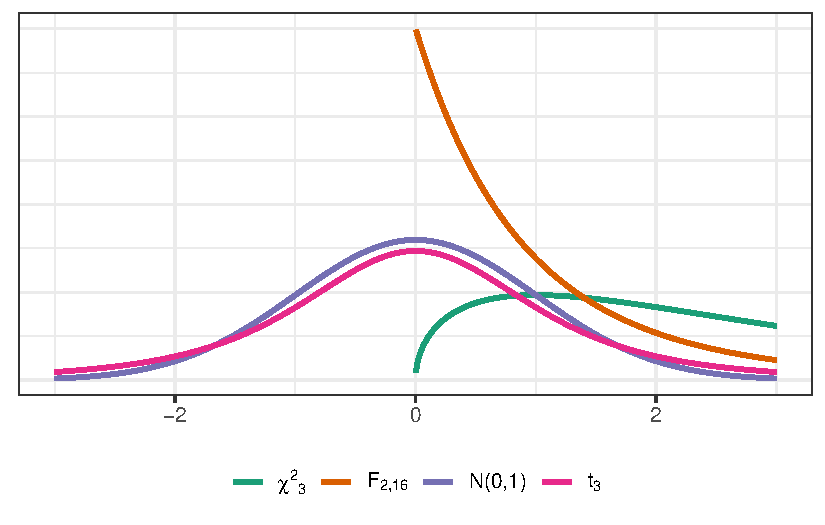
\includegraphics[width=0.8\textwidth,height=\textheight]{./images/fig-randomvariables-comparisons-1.pdf}

}

\caption{\label{fig-randomvariables-comparisons}Comparison of various
common distributions for continuous random variables.}

\end{figure}

The formulas above are ugly, but we will not be working with them
directly. Instead, statistical software have these distributions
embedded. The key idea here is that when we know the model for a
distribution, we can make use of several results about this
distribution.

\begin{tcolorbox}[enhanced jigsaw, title=\textcolor{quarto-callout-tip-color}{\faLightbulb}\hspace{0.5em}{Big Idea}, colbacktitle=quarto-callout-tip-color!10!white, titlerule=0mm, toptitle=1mm, breakable, bottomtitle=1mm, colframe=quarto-callout-tip-color-frame, opacitybacktitle=0.6, bottomrule=.15mm, arc=.35mm, toprule=.15mm, colback=white, rightrule=.15mm, coltitle=black, leftrule=.75mm, left=2mm, opacityback=0]

Some probability models occur so frequently that we give them names for
easy reference. Some models are common for modeling the population, in
which case they are defined in terms of unknown parameters to be
estimated. Some models are used, not to model a population, but to model
other distributions that occur in statistical practice.

\end{tcolorbox}

\hypertarget{transformations-of-a-random-variable}{%
\section{Transformations of a Random
Variable}\label{transformations-of-a-random-variable}}

Occasionally, we are interested in a transformation of a particular
characteristic. That is, we have a model for the distribution of \(X\),
but we are interested in \(Y = g(X)\). In this section, we examine one
method for determining the density of \(Y\) from the density of \(X\).

While there various approaches to this problem, we find this method the
most reliable. Further, it does not require the memorization of a
formula, but instead builds on fundamental ideals. This is known as the
\textbf{Method of Distribution Functions}.

\begin{definition}[Method of Distribution
Functions]\protect\hypertarget{def-method-of-distribution-functions}{}\label{def-method-of-distribution-functions}

Let \(X\) be a continuous random variable with density \(f\) and
cumulative distribution function \(F\). Consider \(Y = h(X)\). The
following process provides the density function \(g\) of \(Y\) by first
finding its cumulative distribution function \(G\).

\begin{enumerate}
\def\labelenumi{\arabic{enumi}.}
\tightlist
\item
  Find the set \(A\) for which \(h(X) \leq t\) if and only if
  \(X \in A\).
\item
  Recognize that
  \(G(y) = Pr(Y \leq y) = Pr\left(h(X) \leq y\right) = Pr(X \in A)\).
\item
  If interested in \(g(y)\), note that
  \(g(y) = \frac{\partial}{\partial y} G(y)\).
\end{enumerate}

\end{definition}

When \(h\) is a strictly monotone function (unique inverse exists), then
step 1-2 is much easier because we can apply \(h^{-1}\). In step 2 of
the above process, the final expression is often left in terms of \(F\),
the CDF of \(X\); then, when we find the density in step 3, we can apply
the chain rule (avoiding the need to actually have an expression for
\(F\)).

\begin{example}[Transformation of a Random
Variable]\protect\hypertarget{exm-transformations}{}\label{exm-transformations}

Previously, we posited the following model for the distribution of the
cost of a diamond sold in the US:

\[f(x) = \frac{1}{\sigma} e^{-x/\sigma} \qquad x > 0\]

for some \(\sigma > 0\). As cost is generally a heavily skewed variable,
we may be interested in taking the (natural) logarithm before proceeding
with an analysis. Find the density of \(Y = \log(X)\).

\end{example}

\begin{solution}

We note that \(\log(x)\) is a strictly monotone function. Therefore, we
have that

\[
\begin{aligned}
  G(y) &= Pr(Y \leq y) \\
    &= Pr(\log(X) \leq y) \\
    &= Pr\left(X \leq e^y\right).
\end{aligned}
\]

Just to place this within the method described above, since
\(\log(x) \leq y\) if and only if \(x \leq e^y\), then
\(A = \{t: x \leq e^t\}\). Of course, we didn't really need to identify
this because we were able to apply the inverse of \(\log(x)\) directly
within the probability expression. We now recognize that we have a
probability of the form ``\(X\) less than or equal to something.'' And,
this matches the form of the CDF of \(X\). That is, we have that

\[G(y) = F\left(e^y\right).\]

This completes step 2 of the procedure; we have expressed the CDF of
\(Y\) as a function of the CDF of \(X\). Now, to find the density, we
apply the chain rule.

\[
\begin{aligned}
  g(y) 
    &= \frac{\partial}{\partial y} G(y) \\
    &= \left[\left.\frac{\partial}{\partial x} F(x)\right|_{x = e^y}\right] \frac{\partial}{\partial y} e^y \\
    &= \left[\left. f(x) \right|_{x = e^y}\right] e^y \\
    &= f\left(e^y\right) e^y \\
    &= \frac{1}{\sigma} e^{-e^y/\sigma} e^y
\end{aligned}
\]

which will be valid for all real values of \(y\); that is, the support
of \(Y\) is all real numbers. In line 2 above, we applied the chain rule
to compute the derivative, avoiding the need to explicitly state the CDF
of \(X\).

\end{solution}

\begin{tcolorbox}[enhanced jigsaw, title=\textcolor{quarto-callout-warning-color}{\faExclamationTriangle}\hspace{0.5em}{Warning}, colbacktitle=quarto-callout-warning-color!10!white, titlerule=0mm, toptitle=1mm, breakable, bottomtitle=1mm, colframe=quarto-callout-warning-color-frame, opacitybacktitle=0.6, bottomrule=.15mm, arc=.35mm, toprule=.15mm, colback=white, rightrule=.15mm, coltitle=black, leftrule=.75mm, left=2mm, opacityback=0]

While mathematicians distinguish between a derivative \(\frac{d}{dx}\)
and a partial derivative \(\frac{\partial}{\partial x}\), we do not make
that distinction.

\end{tcolorbox}

\bookmarksetup{startatroot}

\hypertarget{sec-samplingdistributions}{%
\chapter{Sampling Distribution of a
Statistic}\label{sec-samplingdistributions}}

In the previous chapter, we related probability concepts associated with
random variables to their statistical counterparts in data collection.
We introduced the idea of using a density function as a model of the
distribution of a variable within the population. This led to the
observation that the population parameters govern the shape of these
density functions. Further, these parameters are the focal point of
research objectives. In a statistical analysis, the parameters would be
estimated using statistics; in this chapter, we explore how probability
theory helps us to characterize the variability in these statistics ---
which is the key component of statistical inference.

\hypertarget{statistics-and-expectations}{%
\section{Statistics and
Expectations}\label{statistics-and-expectations}}

The goal of statistics is to use a sample to say something about the
underlying population. Consider the following research objective:

\begin{quote}
Estimate the cost (in US dollars) of a diamond for sale in the United
States.
\end{quote}

No researcher would believe that measuring the cost of a single diamond
would be sufficient to address the above research objective. Instead, we
would consider taking a sample of \(n\) diamonds and measuring the cost
of each. We can represent the cost we will record (note the use of the
future tense) as \(X_1, X_2, \dotsc, X_n\), where \(X_i\) is the cost of
the \(i\)-th diamond we will measure. Collecting data on a sample
requires that we deal with at least \(n\) random variables (one
measurement for each of the observations in our sample).

In almost every analysis, we compute a numerical summary of the data.
For example, the sample mean takes the form

\[\bar{x} = \frac{1}{n} \sum_{i=1}^{n} x_i.\]

\begin{tcolorbox}[enhanced jigsaw, title=\textcolor{quarto-callout-note-color}{\faInfo}\hspace{0.5em}{Note}, colbacktitle=quarto-callout-note-color!10!white, titlerule=0mm, toptitle=1mm, breakable, bottomtitle=1mm, colframe=quarto-callout-note-color-frame, opacitybacktitle=0.6, bottomrule=.15mm, arc=.35mm, toprule=.15mm, colback=white, rightrule=.15mm, coltitle=black, leftrule=.75mm, left=2mm, opacityback=0]

While a capital letter denotes a random variable (not yet observed), the
corresponding lowercase letter is used to denote a past observation
(which is no longer random).

\end{tcolorbox}

These numerical summaries, statistics, are functions of the data. So,
prior to when we collect that data, our statistics are functions of
random variables.

\begin{definition}[Statistic]\protect\hypertarget{def-statistic}{}\label{def-statistic}

A statistic is a numerical summary of a sample; it is a function of the
data alone. Prior to collecting data, a statistic is a function of the
data to be collected.

\end{definition}

Definition~\ref{def-statistic} eliminates the possibility of the
statistic being a function of the underlying \emph{parameters};
certainly, the behavior of the statistic is determined by the
parameters, but the computation of a statistic should not require
knowledge of the parameter once the data is collected.

Definition~\ref{def-statistic} highlights the need to study functions
and combinations of random variables. If you recall,
Theorem~\ref{thm-expectation} introduced the idea of expectation as a
linear operator. The result, for a single random variable, is nearly
intuitive. If expectation is associated with integration (as defined in
Definition~\ref{def-mean}), then expectations should adopt the
properties of integration, including linearity. The generalization of
this result is extremely important within statistics.

\begin{theorem}[Linearity of
Expectations]\protect\hypertarget{thm-linearity-of-expectations}{}\label{thm-linearity-of-expectations}

For random variables \(X_1, X_2, \dotsc, X_n\), constants
\(a_1, a_2, \dotsc, a_n\) and real-valued functions
\(g_1, g_2, \dotsc, g_n\), we have that

\[E\left[\sum_{i=1}^{n} a_i g\left(X_i\right)\right] = \sum_{i=1}^{n} a_i E\left[g\left(X_i\right)\right].\]

\end{theorem}

The importance of Theorem~\ref{thm-linearity-of-expectations} is seen in
determining the expectation of the sample mean.

\begin{example}[Mean of the Sample
Mean]\protect\hypertarget{exm-mean-xbar}{}\label{exm-mean-xbar}

Let \(X_1, X_2, \dotsc, X_n\) be random variables representing
observations from a sample that will be collected. Define the sample
mean of that future sample to be

\[\bar{X} = \frac{1}{n} \sum_{i=1}^{n} X_i.\]

Determine \(E\left(\bar{X}\right)\).

\end{example}

Before addressing the prompt in Example~\ref{exm-mean-xbar}, we note
that \emph{before collecting the data}, statistics, like the sample
mean, is a function of random variables and is therefore itself a random
variable! And, all random variables have distributions, and they have
parameters that govern the shape of that distribution.
Example~\ref{exm-mean-xbar} is focused on the mean of the distribution.

\begin{solution}

Applying Theorem~\ref{thm-linearity-of-expectations}, we have

\[
\begin{aligned}
  E\left(\bar{X}\right)
    &= E\left(\frac{1}{n} \sum_{i=1}^{n} X_i\right) \\
    &= \frac{1}{n} \sum_{i=1}^{n} E\left(X_i\right)
\end{aligned}
\]

If we assume that each \(X_i\) is taken from the same population, then
\(E\left(X_i\right) = \mu\), the population mean, for some constant
\(\mu\). Therefore, we have that

\[E\left(\bar{X}\right) = \frac{1}{n} \sum_{i=1}^{n} \mu = \mu.\]

\end{solution}

Theorem~\ref{thm-linearity-of-expectations} discusses how expectations
work with linear combinations; we have a similar result for variances.
However, there is a particular caveat.

\begin{theorem}[Variance of the Sum of Independent Random
Variables]\protect\hypertarget{thm-variance-independent-sum}{}\label{thm-variance-independent-sum}

Let \(X_1, X_2, \dotsc, X_n\) be independent random variables, and
define constants \(a_1, a_2, \dotsc, a_n\) and real-valued functions
\(g_1, g_2, \dotsc, g_n\). Then,

\[Var\left[\sum_{i=1}^{n} a_i g\left(X_i\right)\right] = \sum_{i=1}^{n} a^2_i Var\left[g\left(X_i\right)\right].\]

\end{theorem}

Comparing Theorem~\ref{thm-linearity-of-expectations} to
Theorem~\ref{thm-variance-independent-sum}, we see that while the
expectation always move through sums, the variance only does so when the
random variables are independent.

\begin{definition}[Independence]\protect\hypertarget{def-independence}{}\label{def-independence}

Random variables \(X_1, X_2, \dotsc, X_n\) are said to be mutually
independent (or just ``independent'') if and only if

\[Pr\left(X_1 \in A_1, X_2 \in A_2, \dotsb, X_n \in A_n\right) = \prod_{i=1}^{n} Pr\left(X_i \in A_i\right),\]

where \(A_1, A_2, \dotsc, A_n\) are arbitrary sets.

\end{definition}

\begin{tcolorbox}[enhanced jigsaw, title=\textcolor{quarto-callout-note-color}{\faInfo}\hspace{0.5em}{Note}, colbacktitle=quarto-callout-note-color!10!white, titlerule=0mm, toptitle=1mm, breakable, bottomtitle=1mm, colframe=quarto-callout-note-color-frame, opacitybacktitle=0.6, bottomrule=.15mm, arc=.35mm, toprule=.15mm, colback=white, rightrule=.15mm, coltitle=black, leftrule=.75mm, left=2mm, opacityback=0]

For those not familiar, \(\prod_{i=1}^n a_i\) is the \emph{product
operator}. It is analogous to \(\sum_{i=1}^{n} a_i\), but uses products
instead of sums.

\end{tcolorbox}

Essentially, a random variable \(X\) is said to be independent of \(Y\)
if the likelihood that \(X\) takes a particular value is the same
regardless of the value \(Y\) takes.

Consider taking a sample of \(n\) diamonds to address our above research
objective. It seems reasonable that the cost of one diamond does not
depend on the cost of another. That allows us to assume the values we
collect will be independent; that is, the random variables we use to
represent these costs are independent of one another. It also seems
natural to assume that each diamond we select comes from the same
underlying population. These two attributes together form the basis of
what we mean by a ``random sample.''

\begin{definition}[Random
Sample]\protect\hypertarget{def-random-sample}{}\label{def-random-sample}

A random sample of size \(n\) refers to a collection of \(n\) random
variables \(X_1, X_2, \dotsc, X_n\) such that the random variables are
mutually independent, and the distribution of each random variable is
identical.

We say \(X_1, X_2, \dotsc, X_n\) are independent and identically
distributed, abbreviated IID. We might also write this as
\(X_i \stackrel{\text{IID}}{\sim} f\) for some density \(f\).

\end{definition}

\begin{tcolorbox}[enhanced jigsaw, title=\textcolor{quarto-callout-warning-color}{\faExclamationTriangle}\hspace{0.5em}{Warning}, colbacktitle=quarto-callout-warning-color!10!white, titlerule=0mm, toptitle=1mm, breakable, bottomtitle=1mm, colframe=quarto-callout-warning-color-frame, opacitybacktitle=0.6, bottomrule=.15mm, arc=.35mm, toprule=.15mm, colback=white, rightrule=.15mm, coltitle=black, leftrule=.75mm, left=2mm, opacityback=0]

Let \(X\) and \(Y\) be identically distributed random variables. This
does not mean that \(X = Y\). That is, the two random variables need not
take on the same value. Instead, identically distributed means the
density function of the two random variables are the same. As a result,
they share the same mean, variance, etc. That is, their distributions
are the same, not their value.

\end{tcolorbox}

\begin{example}[Variance of the Sample
Mean]\protect\hypertarget{exm-var-xbar}{}\label{exm-var-xbar}

Let \(X_1, X_2, \dotsc, X_n\) be a random sample of size \(n\) from a
population with a variance of \(\sigma^2\). Define the sample mean of
that future sample to be

\[\bar{X} = \frac{1}{n} \sum_{i=1}^{n} X_i.\]

Determine \(Var\left(\bar{X}\right)\).

\end{example}

\begin{solution}

Since \(X_1, X_2, \dotsc, X_n\) form a random sample; we know that they
are mutually independent. Therefore,
Theorem~\ref{thm-variance-independent-sum} gives

\[
\begin{aligned}
  Var\left(\bar{X}\right)
    &= Var\left(\frac{1}{n} \sum_{i=1}^{n} X_i\right) \\
    &= \frac{1}{n^2} \sum_{i=1}^{n} Var\left(X_i\right) \\
    &= \frac{1}{n^2} \sum_{i=1}^{n} \sigma^2 \\
    &= \sigma^2 / n.
\end{aligned}
\]

\end{solution}

\begin{tcolorbox}[enhanced jigsaw, title=\textcolor{quarto-callout-warning-color}{\faExclamationTriangle}\hspace{0.5em}{Warning}, colbacktitle=quarto-callout-warning-color!10!white, titlerule=0mm, toptitle=1mm, breakable, bottomtitle=1mm, colframe=quarto-callout-warning-color-frame, opacitybacktitle=0.6, bottomrule=.15mm, arc=.35mm, toprule=.15mm, colback=white, rightrule=.15mm, coltitle=black, leftrule=.75mm, left=2mm, opacityback=0]

It is important to remember that Example~\ref{exm-mean-xbar} and
Example~\ref{exm-var-xbar} describe the mean and variance of the sample
mean \emph{prior to} collecting data. Once the data is collected, the
sample mean has no distribution. Once the data is collected, a statistic
is simply a number.

\end{tcolorbox}

There is one additional result for independent random variables that we
should keep in mind.

\begin{definition}[Expectation of a Product of Independent Random
Variables]\protect\hypertarget{def-product-expectations}{}\label{def-product-expectations}

Let \(X_1, X_2, \dotsc, X_n\) be independent random variables, then

\[E\left(\prod_{i=1}^n X_i\right) = \prod_{i=1}^{n} E\left(X_i\right).\]

\end{definition}

\hypertarget{sampling-distribution-of-sample-mean}{%
\section{Sampling Distribution of Sample
Mean}\label{sampling-distribution-of-sample-mean}}

Together, Example~\ref{exm-mean-xbar} and Example~\ref{exm-var-xbar}
characterize the center and spread of the distribution of the sample
mean. Since each statistic is a random variable, it has a distribution,
and we call that distribution a \textbf{sampling distribution}.

\begin{definition}[Sampling
Distribution]\protect\hypertarget{def-sampling-distribution}{}\label{def-sampling-distribution}

The distribution of a statistic across repeated samples.

\end{definition}

Note that Definition~\ref{def-sampling-distribution} makes use of the
idea of repeated sampling. Once again, this leans on the frequentist
interpretation of probability
(Definition~\ref{def-frequentist-interpretation}). We are thinking of
the distribution of a statistic as the result of the different values
that could potentially be observed if we were to repeatedly take samples
of the same size.

While Theorem~\ref{thm-linearity-of-expectations} and
Theorem~\ref{thm-variance-independent-sum} allowed us to characterize
the sampling distribution of the sample mean, these results did not
provide information about the shape of the sampling distribution, much
less provide a functional form of the density. To make progress on this
front, we return to another tool introduced in a probability course ---
the \textbf{moment-generating function}.

\begin{definition}[Moment-Generating Function
(MGF)]\protect\hypertarget{def-mgf}{}\label{def-mgf}

For a random variable \(X\), let \(M_X(t)\) be defined as

\[M_X(t) = E\left(e^{tX}\right).\]

If \(M_X(t)\) is defined for all values of \(t\) in some interval about
0, then \(M_X(t)\) is called the moment-generating function (MGF) of
\(X\).

\end{definition}

\begin{tcolorbox}[enhanced jigsaw, title=\textcolor{quarto-callout-note-color}{\faInfo}\hspace{0.5em}{Note}, colbacktitle=quarto-callout-note-color!10!white, titlerule=0mm, toptitle=1mm, breakable, bottomtitle=1mm, colframe=quarto-callout-note-color-frame, opacitybacktitle=0.6, bottomrule=.15mm, arc=.35mm, toprule=.15mm, colback=white, rightrule=.15mm, coltitle=black, leftrule=.75mm, left=2mm, opacityback=0]

When we are working with multiple random variables, it is common to use
a subscript to denote the random variable we are referencing. For
example, \(F_X\) may represent the CDF of the random variable \(X\),
\(f_Y\) denote the density function of the random variable \(Y\), and
\(M_Z(t)\) denote the MGF of the random variable \(Z\).

\end{tcolorbox}

First, we note that the MGF is a function, but not a function of the
random variable. That is, \(M_X(t)\) is not a random variable since it
is the result of taking the expected value of a random variable. Second,
the definition does not guarantee the existence of the MGF for any
particular random variable. That is, there are distributions for which
the MGF is not defined. The power of the MGF is summarized in
\textbf{?@thm-mgf-properties}.

\hypertarget{properties-of-the-moment-generating-function}{%
\section{Properties of the Moment-Generating
Function}\label{properties-of-the-moment-generating-function}}

Let \(X\) be a random variable with moment-generating function
\(M_X(t).\) Then, we have that

\begin{enumerate}
\def\labelenumi{\arabic{enumi}.}
\tightlist
\item
  \(E\left(X^k\right) = M_X^{(k)}(0)\) for all integers \(k\), where
  \(M_X(k)(0)\) is the \(k\)-th derivative of \(M_X(t)\) evaluated at
  \(t = 0\).
\item
  The MGF uniquely defines the random variable. That is, if two random
  variables have the same MGF, then those random variables have the same
  density function.
\end{enumerate}

Consider again our sample of \(n\) diamonds; let's assume it is a random
sample from the population. Suppose we are interested in the total
number of diamonds within this sample that have a ``princess'' cut.
Define the random variable

\[Y_i = \begin{cases} 1 & \text{if i-th diamond has a princess cut} \\ 0 & \text{otherwise}. \end{cases}\]

If we are intersted in the total number of diamonds within the sample
that have a princess cut, we are interested in the statistic
\(\sum_{i=1}^{n} Y_i\). We can use \textbf{?@thm-mgf-properties},
together with our previous results about expectations to derive the
sampling distribution of this statistic.

\begin{example}[Sampling Distribution of a Sum of Bernoulli Random
Variables]\protect\hypertarget{exm-bernoulli-sum}{}\label{exm-bernoulli-sum}

Let \(Y_1, Y_2, \dotsc, Y_n\) be IID random variables from a Bernoulli
distribution with probability \(\theta\). Define

\[Z = \sum_{i=1}^{n} Y_i,\]

the total number of ``successes'' in the random sample. Determine the
sampling distribution of \(Z\).

\end{example}

\begin{solution}

In order to determine the distribution of \(Z\), we find its MGF.

\[
\begin{aligned}
  M_Z(t)
    &= E\left(e^{tZ}\right) \\
    &= E\left(e^{t\sum_{i=1}^{n} Y_i}\right) \\
    &= E\left(\prod_{i=1}^{n} e^{tY_i}\right),
\end{aligned}
\]

where the third line results from recognizing that the product of
exponential terms is the exponential of the sum of the powers. Now,
applying \textbf{?@thm-product-expectation}, we have

\[
\begin{aligned}
  M_Z(t)
    &= \prod_{i=1}^{n} E\left(e^{tY_i}\right) \\
    &= \prod_{i=1}^{n} M_{Y_i}(t) \\
    &= \prod_{i=1}^{n} M_{Y_1}(t)
\end{aligned}
\]

where the last line is the result of the random variables being
identically distributed. Since they have the same distribution, they
must have the same MGF's; therefore, \(M_{Y_i}(t) = M_{Y_1}(t)\) for
each \(i\). Again, we are \emph{not} saying \(Y_i = Y_1\); we are saying
the moment-generating functions of these random variables is equivalent.

Consulting a table to determine the MGF of a Bernoulli random variable,
we have that

\[M_{Y_1}(t) = (1 - \theta) + \theta e^t.\]

Thus, we have that

\[
\begin{aligned}
  M_Z(t)
    &= \prod_{i=1}^{n} M_{Y_1}(t) \\
    &= \left[M_{Y_1}(t)\right]^n \\
    &= \left[(1 - \theta) + \theta e^{t}\right]^n.
\end{aligned}
\]

But, consulting a table of common distributions, we recognize \(M_Z(t)\)
as the moment-generating function of a Binomial distribution with
parameters \(n\) and \(\theta\). Since moment-generating functions
uniquely define a distribution when they exist, we have that
\(Z \sim Bin(n, \theta)\).

\end{solution}

The next chapter will illustrate how we can capitalize on this
information. For this chapter, we simply note that we are able to
characterize how the sum of Bernoulli random variables behaves. We note
that this sampling distribution depends on the unknown parameter
\(\theta\) that also governs the underlying population. In addition, it
depends on the sample size.

\begin{tcolorbox}[enhanced jigsaw, title=\textcolor{quarto-callout-tip-color}{\faLightbulb}\hspace{0.5em}{Big Idea}, colbacktitle=quarto-callout-tip-color!10!white, titlerule=0mm, toptitle=1mm, breakable, bottomtitle=1mm, colframe=quarto-callout-tip-color-frame, opacitybacktitle=0.6, bottomrule=.15mm, arc=.35mm, toprule=.15mm, colback=white, rightrule=.15mm, coltitle=black, leftrule=.75mm, left=2mm, opacityback=0]

The sampling distribution of a statistic depends on both the parameters
from the underlying population as well as the sample size.

\end{tcolorbox}

While the previous example illustrates the process, we admit that it
simply reiterates a fact that we already knew (and noted in
Definition~\ref{def-binomial-distribution}). The utility of the next
result may be a bit more apparent.

\begin{example}[Sampling Distribution of the Sample Mean from a Normal
Population]\protect\hypertarget{exm-normal-mean}{}\label{exm-normal-mean}

Let
\(Y_1, Y_2, \dotsc, Y_n \stackrel{\text{IID}}{\sim} N\left(\mu,\sigma^2\right)\).
Define

\[\bar{Y} = \frac{1}{n}\sum_{i=1}^{n} Y_i,\]

the sample mean. Determine the sampling distribution of \(\bar{Y}\).

\end{example}

\begin{solution}

In order to determine the distribution of \(\bar{Y}\), we find its MGF.

\[
\begin{aligned}
  M_{\bar{Y}}(t)
    &= E\left(e^{t\bar{Y}}\right) \\
    &= E\left(e^{tn^{-1}\sum_{i=1}^{n} Y_i}\right) \\
    &= E\left(\prod_{i=1}^{n} e^{tn^{-1}Y_i}\right) 
\end{aligned}
\]

where the third line results from recognizing that the product of
exponential terms is the exponential of the sum of the powers. Now,
applying \textbf{?@thm-product-expectation}, we have

\[
\begin{aligned}
  M_{\bar{Y}}(t)
    &= \prod_{i=1}^{n} E\left(e^{tn^{-1}Y_i}\right) \\
    &= \prod_{i=1}^{n} M_{Y_i}(t/n) \\
    &= \prod_{i=1}^{n} M_{Y_1}(t/n)
\end{aligned}
\]

where the last line is the result of the random variables being
identically distributed, and the second line makes use of the definition
of the MGF, which can be evaluated at any value, including \(t/n\).
Since they have the same distribution, they must have the same MGF's;
therefore, \(M_{Y_i}(t) = M_{Y_1}(t)\) for each \(i\) and all \(t\).
Again, we are \emph{not} saying \(Y_i = Y_1\); we are saying the
moment-generating functions of these random variables is equivalent.

Consulting a table to determine the MGF of a Normal random variable, we
have that

\[M_{Y_1}(t) = e^{\mu t + (1/2) \sigma^2 t^2}.\]

Thus, we have that

\[
\begin{aligned}
  M_{\bar{Y}}(t)
    &= \prod_{i=1}^{n} M_{Y_1}(t/n) \\
    &= \left[M_{Y_1}(t/n)\right]^n \\
    &= \left[e^{\mu t/n + (1/2) \sigma^2 t^2/n^2}\right]^n \\
    &= e^{\mu t + (1/2)(\sigma^2 / n) t^2}.
\end{aligned}
\]

But, consulting a table of common distributions, we recognize
\(M_{\bar{Y}}(t)\) as the moment-generating function of a Normal
distribution with a mean of \(\mu\) and a variance of \(\sigma^2/n\).
Since moment-generating functions uniquely define a distribution when
they exist, we have that \(\bar{Y} \sim N\left(\mu, \sigma^2/n\right)\).

\end{solution}

We note a difference between Example~\ref{exm-bernoulli-sum} and
Example~\ref{exm-normal-mean}. In Example~\ref{exm-bernoulli-sum}, the
statistic we examined did not estimate a parameter of interest. While
there is nothing wrong with examining the total number of diamonds in a
sample, the statistic itself is dependent on the sample size --- we
would expect a larger value with larger samples. In
Example~\ref{exm-normal-mean}, however, the sample mean is a common
estimate of the population mean. It turns out the sampling distributions
of most estimators (statistics chosen to estimate a parameter) tend to
share similar characteristics.

\begin{tcolorbox}[enhanced jigsaw, title=\textcolor{quarto-callout-note-color}{\faInfo}\hspace{0.5em}{Common Characteristics of Sampling Distributions}, colbacktitle=quarto-callout-note-color!10!white, titlerule=0mm, toptitle=1mm, breakable, bottomtitle=1mm, colframe=quarto-callout-note-color-frame, opacitybacktitle=0.6, bottomrule=.15mm, arc=.35mm, toprule=.15mm, colback=white, rightrule=.15mm, coltitle=black, leftrule=.75mm, left=2mm, opacityback=0]

While not guaranteed, the sampling distribution of many statistics tend
to have the following characteristics:

\begin{enumerate}
\def\labelenumi{\arabic{enumi}.}
\tightlist
\item
  The sampling distribution is centered on the corresponding parameter
  of interest, or the center approaches the corresponding parameter as
  the sample size increases.
\item
  The spread of the sampling distribution is smaller than within the
  population, and the spread decreases as the sample size increases.
\item
  The shape of the sampling distribution differs from that of the
  underlying population, and the sampling distribution becomes more
  bell-shaped as the sample size increases.
\end{enumerate}

Of the three characteristics above, the third is the one most likely to
be broken.

\end{tcolorbox}

Considering Example~\ref{exm-normal-mean}, we see that all three
characteristics hold. First, we see (as we also saw in
Example~\ref{exm-mean-xbar}) that the expected value of the sample mean
is the population mean. When this occurs, we say the estimator is
\textbf{unbiased}.

\begin{definition}[Unbiased]\protect\hypertarget{def-unbiased}{}\label{def-unbiased}

An estimator (statistic) \(\widehat{\theta}\) is said to be unbiased for
the parameter \(\theta\) if

\[E\left(\widehat{\theta}\right) = \theta.\]

\end{definition}

While being unbiased is a good quality in an estimator, it is not
required. For example, the sample standard deviation is not an unbiased
estimator of the population standard deviation, yet it is still a
preferred estimator.

In Example~\ref{exm-normal-mean}, we see that variance of the sample
mean is smaller than the variance of the population by a factor of
\(n\); therefore, as the sample size increases, the variability of the
sample mean decreases. This implies that the sample mean of a large
sample will tend not to stray as far from the population mean as that of
a smaller sample. This is where the notion of ``more data is better''
comes from.

\begin{tcolorbox}[enhanced jigsaw, title=\textcolor{quarto-callout-tip-color}{\faLightbulb}\hspace{0.5em}{Big Idea}, colbacktitle=quarto-callout-tip-color!10!white, titlerule=0mm, toptitle=1mm, breakable, bottomtitle=1mm, colframe=quarto-callout-tip-color-frame, opacitybacktitle=0.6, bottomrule=.15mm, arc=.35mm, toprule=.15mm, colback=white, rightrule=.15mm, coltitle=black, leftrule=.75mm, left=2mm, opacityback=0]

Larger samples result in more reliable statistics.

\end{tcolorbox}

Finally, we see in Example~\ref{exm-normal-mean} that the sampling
distribution of the sample mean is a Normal distribution, which is
bell-shaped. Again, being bell-shaped is not necessarily more
advantageous than any other distribution, but it reinforces the idea
that the statistic tends to be near the parameter of interest across
repeated sampling.

\begin{tcolorbox}[enhanced jigsaw, title=\textcolor{quarto-callout-warning-color}{\faExclamationTriangle}\hspace{0.5em}{Warning}, colbacktitle=quarto-callout-warning-color!10!white, titlerule=0mm, toptitle=1mm, breakable, bottomtitle=1mm, colframe=quarto-callout-warning-color-frame, opacitybacktitle=0.6, bottomrule=.15mm, arc=.35mm, toprule=.15mm, colback=white, rightrule=.15mm, coltitle=black, leftrule=.75mm, left=2mm, opacityback=0]

Remember, these discussions are about the distribution of a statistic
across repeated samples, and so they apply prior to collecting data.
Once we have a sample, the statistic does not have a distribution.

\end{tcolorbox}

Example~\ref{exm-normal-mean} is a really nice result because it tells
us the behavior of a popular statistic; unfortunately, it only applies
to a sample from a population which follows a Normal distribution. More,
it only applies when the population variance is known, which rarely
happens in practice. Theorem~\ref{thm-students-theorem} generalizes the
results to the case when the population variance is unknown.

\begin{theorem}[Student's
Theorem]\protect\hypertarget{thm-students-theorem}{}\label{thm-students-theorem}

Let
\(Y_1, Y_2, \dotsc, Y_n \stackrel{\text{IID}}{\sim} N\left(\mu,\sigma^2\right)\).
Define

\[\bar{Y} = \frac{1}{n}\sum_{i=1}^{n} Y_i\]

to be the sample mean and

\[S^2 = \frac{1}{n-1} \sum_{i=1}^{n} \left(Y_i - \bar{Y}\right)^2\]

to be the sample variance. Then,

\[\frac{\sqrt{n}\left(\bar{Y} - \mu\right)}{S} \sim t_{n-1}.\]

\end{theorem}

To see the impact of estimating the population variance, we recognize
that Example~\ref{exm-normal-mean} gave us that when the population
variance is known

\[\bar{Y} \sim N\left(\mu, \sigma^2/n\right),\]

which can be rewritten as

\[\frac{\sqrt{n}\left(\bar{Y} - \mu\right)}{\sigma} \sim N(0, 1).\]

Therefore, when the population variance is estimated (using the typical
sample variance), we have that the sampling distribution of this
standardized ratio follows a t-distribution instead of a Standard Normal
distribution.

Theorem~\ref{thm-students-theorem} highlights that we often characterize
the distribution of some ``standardized statistic'' (instead of the
statistic that estimates the parameter directly). Exact results like
Example~\ref{exm-normal-mean} and Theorem~\ref{thm-students-theorem} are
quite rare. It is more common for us to rely on approximations to the
sampling distribution, the most famous of which is the Central Limit
Theorem.

\begin{theorem}[Central Limit Theorem
(CLT)]\protect\hypertarget{thm-clt}{}\label{thm-clt}

Let \(X_1, X_2, \dotsc, X_n\) be IID random variables such that
\(E\left(X_i\right) = \mu\) and \(Var\left(X_i\right) = \sigma^2\) for
all \(i\). As \(n\) approaches infinity, the ratio

\[\frac{\sqrt{n}\left(\bar{X} - \mu\right)}{S}\]

behaves like a Standard Normal random variable. That is,

\[Pr\left(\frac{\sqrt{n}\left(\bar{X} - \mu\right)}{S} \leq q\right) \rightarrow Pr(Z \leq q) \qquad \text{as } n \rightarrow \infty\]

where \(q\) is any real number, \(Z \sim N(0, 1)\), \(\bar{X}\) is the
sample mean and \(S^2\) is the sample standard deviation.

\end{theorem}

\begin{tcolorbox}[enhanced jigsaw, title=\textcolor{quarto-callout-note-color}{\faInfo}\hspace{0.5em}{Note}, colbacktitle=quarto-callout-note-color!10!white, titlerule=0mm, toptitle=1mm, breakable, bottomtitle=1mm, colframe=quarto-callout-note-color-frame, opacitybacktitle=0.6, bottomrule=.15mm, arc=.35mm, toprule=.15mm, colback=white, rightrule=.15mm, coltitle=black, leftrule=.75mm, left=2mm, opacityback=0]

``The'' Central Limit Theorem is a misnomer; there are actually several
Central Limit Theorems which differ in their assumptions. The one most
commonly presented in texts uses the population standard deviation
\(\sigma\) instead of the sample standard deviation \(S\) as we have
presented it. The more common presentation is easier to prove, but it is
far less useful in practice (as the population variance is rarely
known). The proof of the version we have presented is beyond the scope
of the course but is more useful in practice.

\end{tcolorbox}

Known as a ``limit'' (or ``asymptotic'') result, Theorem~\ref{thm-clt}
provides an approximation to the sampling distribution. That is, the CLT
states that as the sample size gets large, the Standard Normal
distribution is a good approximation to the true sampling distribution
of this standardized statistic. Of course, that begs the question, ``how
good is the approximation?'' as well as ``how large of a sample is large
enough?'' While we can never address these questions with certainty,
there are some graphical techniques for assessing these questions in
practice.

The huge draw of the CLT is that it applies under vary weak conditions
--- the underlying population has a finite mean and variance. For nearly
any population, we have an approximation for the sampling distribution
of the sample mean.

\begin{tcolorbox}[enhanced jigsaw, title=\textcolor{quarto-callout-note-color}{\faInfo}\hspace{0.5em}{Note}, colbacktitle=quarto-callout-note-color!10!white, titlerule=0mm, toptitle=1mm, breakable, bottomtitle=1mm, colframe=quarto-callout-note-color-frame, opacitybacktitle=0.6, bottomrule=.15mm, arc=.35mm, toprule=.15mm, colback=white, rightrule=.15mm, coltitle=black, leftrule=.75mm, left=2mm, opacityback=0]

The above methods describe the actual sampling distribution. Of course,
because these describe how a statistic behaves across repeated samples,
this is not something we get to observe directly. Instead, the sampling
distribution must be modeled. This is often done by replacing the
parameters in the sampling distribution with the corresponding estimates
from the sample. Therefore, the \emph{model} for the sampling
distribution based on a given sample is really capturing the shape and
spread of the sampling distribution.

\end{tcolorbox}

\hypertarget{bootstrapping}{%
\section{Bootstrapping}\label{bootstrapping}}

In the above sections, we have discussed analytical methods (both exact
and approximation through limit theorems) for the sampling distribution.
Given a set of data, we can also construct a model for the sampling
distribution empirically. As there is no single Central Limit Theorem,
there is no single bootstrapping algorithm. Instead, ``bootstrapping''
refers to the idea of using resampling methods to model a sampling
distribution of a statistic, but the easiest algorithm is defined below.

\begin{definition}[Case-Resampling
Bootstrap]\protect\hypertarget{def-case-bootstrap}{}\label{def-case-bootstrap}

Let \(Y_1, Y_2, \dotsc, Y_n\) be a random sample from an underlying
population, and let \(\theta\) represent a parameter of interest
characterizing the underlying population. Further, define
\(\widehat{\theta} = h(\mathbf{Y})\) be a statistic which estimates the
parameter. The case-resampling bootstrap algorithm proceeds as follows:

\begin{enumerate}
\def\labelenumi{\arabic{enumi}.}
\tightlist
\item
  Take a random sample, with replacement, from the set
  \(\left\{Y_1, Y_2, \dotsc, Y_n\right\}\) of size \(n\). Call these
  values \(Y_1^*, Y_2^*, \dotsc, Y_n^*\). This is known as a bootstrap
  resample.
\item
  Compute \(\widehat{\theta}^* = h\left(\mathbf{Y}^*\right)\) and store
  this value. This is known as a bootstrap statistic.
\item
  Repeat steps 1-2 \(m\) times, for some large value of \(m\) (say
  \(m = 5000\)). Denote \(\widehat{\theta}^*_j\) to be the bootstrap
  statistic from the \(j\)-th bootstrap resample.
\end{enumerate}

The empirical distribution of
\(\widehat{\theta}_1^*, \widehat{\theta}_2^*, \dotsc, \widehat{\theta}_m^*\)
will approximate the shape and spread of the sampling distribution of
the statistic \(h(\mathbf{Y})\).

\end{definition}

While the proof of the efficacy of a bootstrap algorithm is beyond the
scope of this text, we can gain some intuition regarding the process.
Let's start by characterizing the distribution from which the algorithm
resamples --- the distribution of the sample. When we sample, with
replacement, from the original sample, only \(n\) values are possible
\(\left(Y_1, Y_2, \dotsc, Y_n\right)\). And, each value will be selected
with probability \(1/n\). That is, we have that

\[Pr\left(Y_i^* = u\right) = \frac{1}{n} \qquad u \in \left\{Y_1, Y_2, \dotsc, Y_n\right\}.\]

The mean of this distribution is represented by

\[\bar{Y} = \frac{1}{n} \sum_{i=1}^{n} Y_i,\]

and the variance of this distribution is

\[S^2_n = \frac{1}{n} \sum_{i=1}^{n} \left(Y_i - \bar{Y}\right)^2.\]

We divide by \(n\) instead of \(n - 1\) because since we are treating
the original sample as a population from which to be sampled, we rely on
the formulas from Chapter~\ref{sec-randomvariables}.

If \(\widehat{\theta} = \bar{Y}\), then we have that the sampling
distribution of \(\widehat{\theta}^* = n^{-1}\sum_{i=1}^{n} Y_i^*\) will
have a mean of

\[E\left[\frac{1}{n} \sum_{i=1}^{n} Y_i^*\right] = \bar{Y}\]

and a variance of

\[Var\left[\frac{1}{n} \sum_{i=1}^{n} Y_i^*\right] = \frac{S_n^2}{n}.\]

These are the direct application of Example~\ref{exm-mean-xbar} and
Theorem~\ref{thm-variance-independent-sum}. And, if \(n\) is large
enough, we would expect the resulting empirical distribution to
approximate that of a Normal distribution as a result of the CLT. This
highlights that \emph{models} of the sampling distribution tend to have
similar characteristics to that of sampling distributions.

\begin{tcolorbox}[enhanced jigsaw, title=\textcolor{quarto-callout-note-color}{\faInfo}\hspace{0.5em}{Common Characteristics of Models for Sampling Distributions}, colbacktitle=quarto-callout-note-color!10!white, titlerule=0mm, toptitle=1mm, breakable, bottomtitle=1mm, colframe=quarto-callout-note-color-frame, opacitybacktitle=0.6, bottomrule=.15mm, arc=.35mm, toprule=.15mm, colback=white, rightrule=.15mm, coltitle=black, leftrule=.75mm, left=2mm, opacityback=0]

While not guaranteed, the model of a sampling distribution of many
statistics tend to have the following characteristics:

\begin{enumerate}
\def\labelenumi{\arabic{enumi}.}
\tightlist
\item
  The model of the sampling distribution is centered on the statistic
  from the original sample, or the center of the model approaches the
  statistic from the original sample as the sample size increases.
\item
  The spread of the model of the sampling distribution is smaller than
  within the sample, and the spread decreases as the sample size
  increases.
\item
  The shape of the model of the sampling distribution differs from that
  of the sample, and the model of the sampling distribution becomes more
  bell-shaped as the sample size increases.
\end{enumerate}

Of the three characteristics above, the third is the one most likely to
be broken.

\end{tcolorbox}

\hypertarget{application}{%
\section{Application}\label{application}}

Consider the following research objective:

\begin{quote}
Estimate the cost (in US dollars) of a diamond for sale in the United
States.
\end{quote}

As stated, this is an ill-posed objective as it is not centered on a
parameter. We might refine it to be

\begin{quote}
Estimate the average cost (in US dollars) of a diamond for sale in the
United States.
\end{quote}

We have a large (\(n = 53940\)) sample of diamonds at our disposal that
can be used to address this research objective. A plot of the sample is
shown in Figure~\ref{fig-samplingdistributions-sample}.

\begin{figure}

{\centering 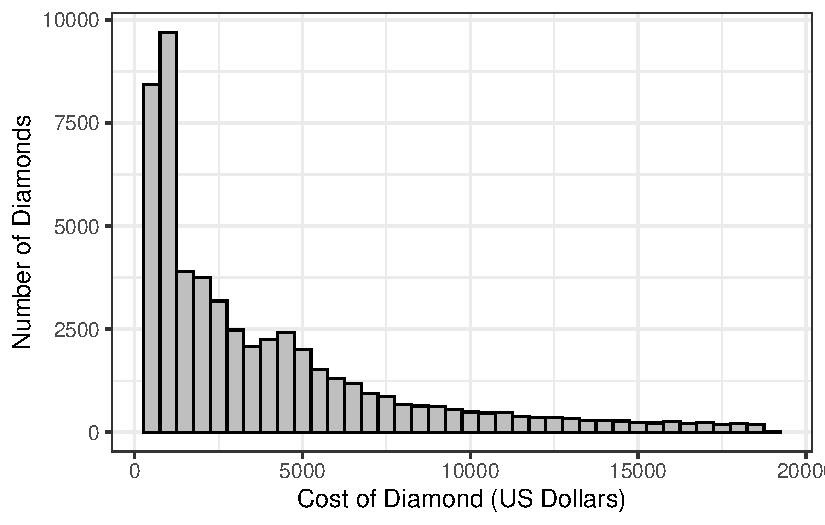
\includegraphics[width=0.8\textwidth,height=\textheight]{./images/fig-samplingdistributions-sample-1.pdf}

}

\caption{\label{fig-samplingdistributions-sample}Distribution of the
cost of a diamond sold in the United States.}

\end{figure}

Using the sample, we conduct 5000 bootstrap replications, each time
computing the sample mean. The bootstrap sampling distribution is shown
in Figure~\ref{fig-samplingdistributions-bootstrap}. We have overlayed
the model suggested by the CLT as well. Observe that even though the
sample was skewed to the right, the model for the sampling distribution
is bell-shaped. The center of our model is the observed sample mean of
3933, and the spread of the sampling distribution is much smaller than
that observed in the sample. With a large sample size, we see that the
empirical model of the sampling distribution is very similar to that
suggested by the CLT.

\begin{tcolorbox}[enhanced jigsaw, title=\textcolor{quarto-callout-note-color}{\faInfo}\hspace{0.5em}{Note}, colbacktitle=quarto-callout-note-color!10!white, titlerule=0mm, toptitle=1mm, breakable, bottomtitle=1mm, colframe=quarto-callout-note-color-frame, opacitybacktitle=0.6, bottomrule=.15mm, arc=.35mm, toprule=.15mm, colback=white, rightrule=.15mm, coltitle=black, leftrule=.75mm, left=2mm, opacityback=0]

Bootstrapping can be used to qualitatively assess whether the CLT is
appropriate for a particular sample. Of course, if we have gone through
the effort of constructing an empirical model, we would likely rely on
the empirical model.

\end{tcolorbox}

Figure~\ref{fig-samplingdistributions-bootstrap} does not include the
results from Theorem~\ref{thm-students-theorem}; the rationale for
excluding this result is that a quick glance at
Figure~\ref{fig-samplingdistributions-sample} is enough to convince us
that the underlying population does not follow a Normal distribution;
therefore, those results are inappropriate.

\begin{figure}

{\centering 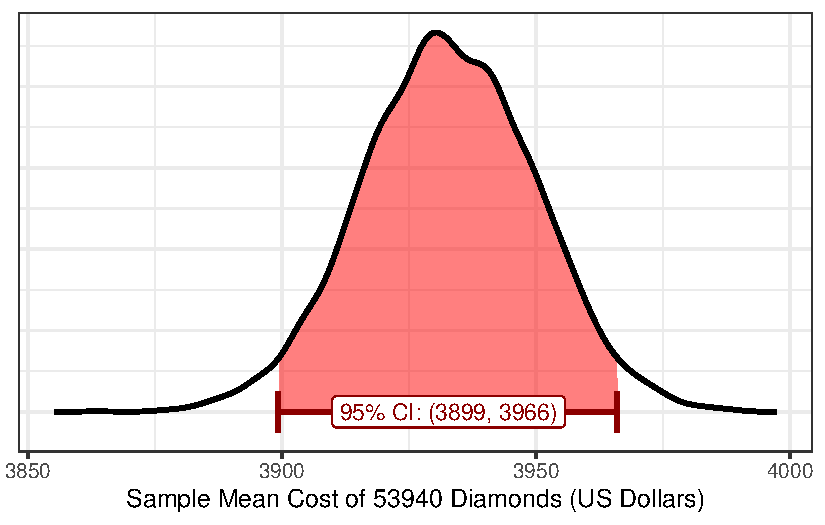
\includegraphics[width=0.8\textwidth,height=\textheight]{./images/fig-samplingdistributions-bootstrap-1.pdf}

}

\caption{\label{fig-samplingdistributions-bootstrap}Bootstrap sampling
distribution of the sample mean cost of a diamond based on the available
data. 5000 bootstrap replicates were used.}

\end{figure}

The next chapter considers ways of using the above tools to perform
inference.

\bookmarksetup{startatroot}

\hypertarget{sec-inference}{%
\chapter{Inference for a Population Mean}\label{sec-inference}}

In the previous chapter, we examined properties of sampling
distribution, with particular attention paid to the sampling
distribution of the sample mean. We also discussed both analytical and
empirical methods for modeling the sampling distribution of a statistic.
In this chapter, we build on those results to conduct inference on a
parameter.

\hypertarget{confidence-intervals}{%
\section{Confidence Intervals}\label{confidence-intervals}}

Sampling distributions characterize the variability in a statistic
across repeated samples. That is, we expect the statistic to differ from
one sample to another. However, what the sampling distribution reveals
is that the degree to which these statistics vary, and the degree to
which they vary from the corresponding parameter, is quantifiable. This
is how sampling distributions are used in a probability course --- given
an underlying population, determine the probability that the sample mean
exceeds a particular value. In statistics, however, we want to go in the
other direction --- given a set of data, determine a suitable interval
of estimates for the parameter.

Figure~\ref{fig-inference-samplingdistribution} accompanies the
``forward'' direction that would accompany a probability problem. Given
the sampling distribution, we would be 95\% sure the statistic would
fall within \(d\) units of the parameter \(\theta\), as illustrated by
the shaded region.

\begin{figure}

{\centering 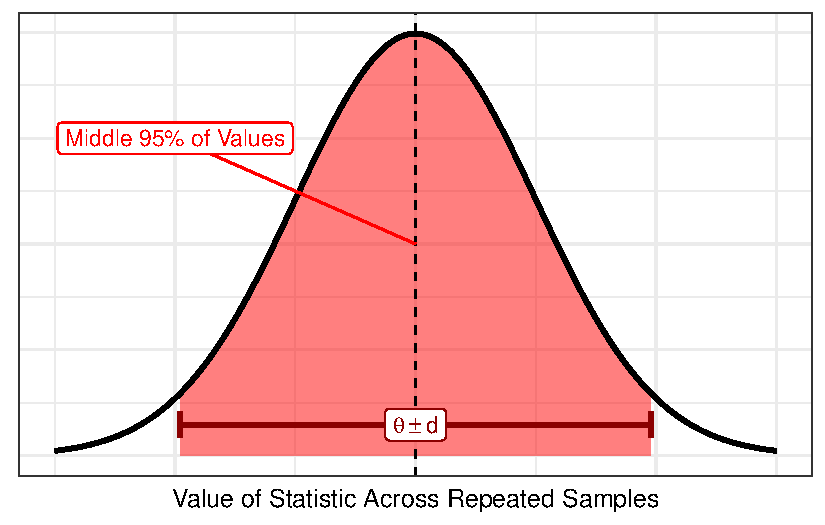
\includegraphics[width=0.8\textwidth,height=\textheight]{./images/fig-inference-samplingdistribution-1.pdf}

}

\caption{\label{fig-inference-samplingdistribution}Illustration of using
a sampling distribution to determine the values of a statistic we would
likely observe in a new sample.}

\end{figure}

Given a sample, we want to ``reverse engineer'' the problem. That is,
the sampling distribution tells us that the statistic would likely not
fall more than \(d\) units from the parameter. Therefore, if we take a
sample from the underlying population and compute a statistic, we would
expect the parameter to be within \(d\) units of this statistic. This is
illustrated in Figure~\ref{fig-inference-model}, where the difference is
that the model for the sampling distribution is centered on the
statistic. We call this a \textbf{confidence interval}.

\begin{figure}

{\centering 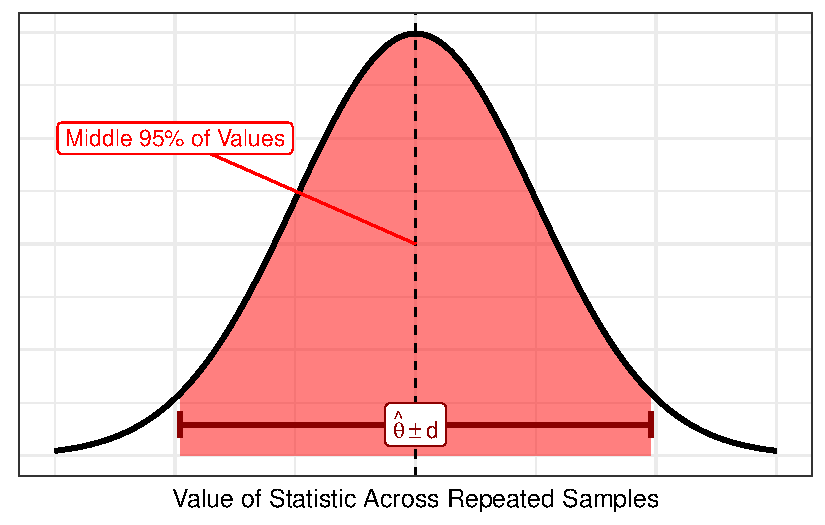
\includegraphics[width=0.8\textwidth,height=\textheight]{./images/fig-inference-model-1.pdf}

}

\caption{\label{fig-inference-model}Illustration of using a model for
the sampling distribution to determine the values of the parameter that
are consistent with the observed sample.}

\end{figure}

\begin{definition}[Confidence
Interval]\protect\hypertarget{def-confidence-interval}{}\label{def-confidence-interval}

Consider repeatedly taking samples \(\mathbf{Y}\) of size \(n\) from a
population characterized by the parameter \(\theta\). The interval
\(\left(h_1(\mathbf{Y}), h_2(\mathbf{Y})\right)\) is said to be a
\(100c\)\% confidence interval if

\[Pr\left(h_1(\mathbf{Y}) \leq \theta \leq h_2(\mathbf{Y})\right) = c.\]

\end{definition}

\begin{tcolorbox}[enhanced jigsaw, title=\textcolor{quarto-callout-warning-color}{\faExclamationTriangle}\hspace{0.5em}{Warning}, colbacktitle=quarto-callout-warning-color!10!white, titlerule=0mm, toptitle=1mm, breakable, bottomtitle=1mm, colframe=quarto-callout-warning-color-frame, opacitybacktitle=0.6, bottomrule=.15mm, arc=.35mm, toprule=.15mm, colback=white, rightrule=.15mm, coltitle=black, leftrule=.75mm, left=2mm, opacityback=0]

It is important to note that in the definition of a confidence interval,
the statistics \(h_1(\mathbf{Y})\) and \(h_2(\mathbf{Y})\) are the
random variables; the parameter \(\theta\) is fixed. That is, it is the
\emph{interval} that is moving across the repeated samples, not the
parameter. Instead of saying ``the probability the parameter is within
the interval,'' we would say ``the probability the interval captures the
parameter.'' While this may seem subtle, it is important for correctly
interpreting the interval.

\end{tcolorbox}

Notice that in the definition of a confidence interval depends on
repeated sampling. Once we have a sample, probability no longer makes
sense; the interval either captures the parameter or it does not, but
our ignorance of the result does not warrant a probability statement.
This is a direct result of our interpretation of probability
(Definition~\ref{def-frequentist-interpretation}).

\begin{example}[CI for Sample Mean Using
CLT]\protect\hypertarget{exm-ci-clt}{}\label{exm-ci-clt}

Let \(Y_1, Y_2, \dotsc, Y_n\) be a large random sample from a population
with a finite mean \(\mu\) and variance \(\sigma^2\). Develop a
\(100c\)\% confidence interval for the population mean \(\mu\).

\end{example}

\begin{solution}

Define \(z_{0.5(1 + c)}\) to be the value such that

\[Pr\left(Z \leq z_{0.5(1+c)}\right) = 0.5(1 + c)\]

for any \(0 < c < 1\) where \(Z \sim N(0, 1)\). Then, we know that

\[c = Pr\left(-z_{0.5(1+c)} \leq Z \leq z_{0.5(1+c)}\right)\]

because of the symmetry of the Normal distribution. Defining \(\bar{Y}\)
and \(S\) to be the sample mean and standard deviation from the sample,
from the CLT, we know that the ratio
\(\frac{\sqrt{n}\left(\bar{Y} - \mu\right)}{S}\) can be approximated by
a Standard Normal distribution. That is, probability statements about
this ratio are equivalent to probability statements about a Standard
Normal random variable. Therefore, we have

\[c = Pr\left(-z_{0.5(1+c)} \leq \frac{\sqrt{n}\left(\bar{Y} - \mu\right)}{S} \leq z_{0.5(1+c)}\right).\]

We now rearranging terms, we have

\[
\begin{aligned}
  c 
    &= Pr\left(-z_{0.5(1+c)} \leq \frac{\sqrt{n}\left(\bar{Y} - \mu\right)}{S} \leq z_{0.5(1+c)}\right) \\
    &= Pr\left(-z_{0.5(1+c)}\frac{S}{\sqrt{n}} \leq \left(\bar{Y} - \mu\right) \leq z_{0.5(1+c)}\frac{S}{\sqrt{n}}\right) \\
    &= Pr\left(\bar{Y} - z_{0.5(1+c)} \frac{S}{\sqrt{n}} \leq \mu \leq \bar{Y} + z_{0.5(1+c)} \frac{S}{\sqrt{n}}\right).
\end{aligned}
\]

Defining \(h_1(\mathbf{Y}) = \bar{Y} - z_{0.5(1+c)}\frac{S}{\sqrt{n}}\)
and \(h_2(\mathbf{Y}) = \bar{Y} + z_{0.5(1+c)}\frac{S}{\sqrt{n}}\), we
have identified an interval
\(\left(h_1(\mathbf{Y}), h_2(\mathbf{Y})\right)\) that satisfies the
definition of a \(100c\)\% confidence interval.

\end{solution}

Consider the following research objective:

\begin{quote}
Estimate the average cost (in US dollars) of a diamond for sale in the
United States.
\end{quote}

In the previous chapter, we saw that the CLT could be used to model the
sampling distribution of the sample mean using the available data.
Applying the result of Example~\ref{exm-ci-clt}, we have that a 95\%
confidence interval for the average cost of a diamond is given by

\[
\begin{aligned}
  \bar{y} &\pm z_{0.925} \left(s / \sqrt{n}\right) \\
  3932.8 &\pm (1.96) (3989.4 / \sqrt{53940}) \\
  (3899&,\ 3966).
\end{aligned}
\]

While Example~\ref{exm-ci-clt} provided a formula for a confidence
interval using the CLT, we can also develop a confidence interval in the
same spirit from an empirical model. Simply define \(h_1(\mathbf{Y})\)
and \(h_2(\mathbf{Y})\) to be the 2.5-th and 97.5-th percentiles from
the empirical sampling distribution. Then, we will have a valid 95\%
confidence interval. \textbf{?@fig-inference-bootstrap} illustrates the
95\% CI using the same data.

\begin{figure}

{\centering 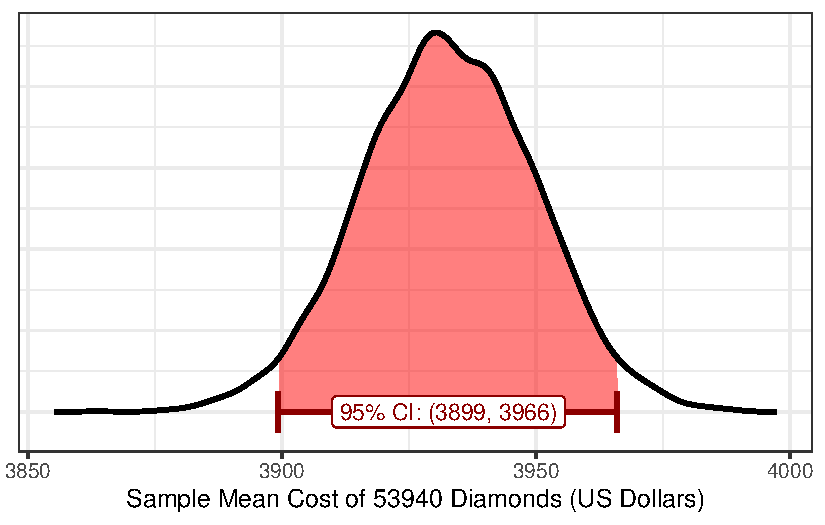
\includegraphics[width=0.8\textwidth,height=\textheight]{./images/fig-samplingdistributions-bootstrap-1.pdf}

}

\caption{\label{fig-samplingdistributions-bootstrap}Bootstrap sampling
distribution of the sample mean cost of a diamond based on the available
data. 5000 bootstrap replicates were used.}

\end{figure}

Not surprisingly, since we saw in the last chapter that the empirical
model and the CLT were extremely similar, the 95\% CI from the empirical
model matches the 95\% CI given by the CLT.

\hypertarget{null-distributions-and-p-values}{%
\section{Null Distributions and
P-Values}\label{null-distributions-and-p-values}}

The disciplines of probability and statistics blend together most
naturally when performing a hypothesis test. In
Chapter~\ref{sec-samplingdistributions}, we examined sampling
distributions of a statistic, with particular attention paid to the
sample mean. We had to transition to modeling these sampling
distributions using data since the population parameters, which also
characterize the sampling distribution of the statistic, are unknown.
When we are performing a hypothesis test, however, the null distribution
specifies a particular value of the unknown parameter(s); this then
allows us to make use of our models directly! This is known as a
\textbf{null distribution}.

\begin{definition}[Null
Distribution]\protect\hypertarget{def-null-distribution}{}\label{def-null-distribution}

Distribution of a statistic under a hypothesized value of the population
parameter(s).

\end{definition}

Let's return to our investigation of diamond prices. Suppose we are
interested in the following research question:

\begin{quote}
Is it reasonable that the average cost (in US dollars) of a diamond is
\$3900? Or, does the sample provide evidence that the average cost of a
diamond exceeds \$3900?
\end{quote}

Letting \(\theta\) represent the average cost (in US dollars) of a
diamond, the above research question can be captured using the following
hypotheses:

\[H_0: \theta \leq 3900 \qquad \text{vs.} \qquad H_1: \theta > 3900.\]

From the CLT, we have that the sampling distribution of the ratio

\[\frac{\sqrt{n}\left(\bar{Y} - \theta\right)}{S}\]

can be approximated by a Standard Normal distribution, where \(\bar{Y}\)
and \(S\) represent the sample mean and standard deviation,
respectively. In the above ratio, \(\theta\) is unknown. However,
\emph{if we are willing to assume the above null hypothesis is true},
then we know that \(\theta = 3900\).

\begin{tcolorbox}[enhanced jigsaw, title=\textcolor{quarto-callout-note-color}{\faInfo}\hspace{0.5em}{Note}, colbacktitle=quarto-callout-note-color!10!white, titlerule=0mm, toptitle=1mm, breakable, bottomtitle=1mm, colframe=quarto-callout-note-color-frame, opacitybacktitle=0.6, bottomrule=.15mm, arc=.35mm, toprule=.15mm, colback=white, rightrule=.15mm, coltitle=black, leftrule=.75mm, left=2mm, opacityback=0]

When working with a one-sided hypothesis, ``assuming the null
hypothesis'' always considers the boundary of the interval. The idea
here is that if we can establish evidence against this boundary, then we
can establish evidence against any other value represented in the null
hypothesis.

\end{tcolorbox}

That is, \emph{if the null hypothesis is true}, then we have that the
sampling distribution of the ratio

\[\frac{\sqrt{n}\left(\bar{Y} - 3900\right)}{S}\]

can be approximated by a Standard Normal distribution. Essentially, we
are using the CLT combined with the knowledge provided by the null
hypothesis about the parameters. That is, we really are discussing the
\emph{null distribution}. Now, we can use this distribution to make
probabilistic statements. For example, we might ask the following
question:

\begin{quote}
Assuming the null hypothesis is true, what is the probability that the
ratio \(\frac{\sqrt{n}\left(\bar{Y} - 3900\right)}{S}\) would meet or
exceed 1.909?
\end{quote}

This is a straight-forward probability problem. Observe that

\[
\begin{aligned}
  Pr\left(\frac{\sqrt{n}\left(\bar{Y} - 3900\right)}{S} \geq 1.909\right)
    &= Pr(Z \geq 1.909) \\
    &= 0.0281
\end{aligned}
\]

where \(Z \sim N(0, 1)\). That is, assuming the mean cost of a diamond
is \$3900, there is only a 2.81\% chance that we would observe a ratio
of at least 1.909. However, using the data we obtained, we find that the
ratio we observed in our sample was 1.909, where we use the observed
sample mean and standard deviation in the computation. That is, if the
average cost of a diamond is \$3900, if we were to repeat the study,
there is only a 2.81\% chance that we would observe data that would
provide a ratio as extreme or more so than that observed. Further,
larger values of this ratio are more consistent with the alternative
hypothesis (average costs larger than \$3900). So, if the average cost
of a diamond is \$3900, there is only a 2.81\% chance that we would
observe data as consistent or more so with the alternative hypothesis as
that observed. This is known as a \textbf{p-value}.

\begin{definition}[P-value]\protect\hypertarget{def-pvalue}{}\label{def-pvalue}

The probability, assuming the null hypothesis is true, that we would
observe a statistic, by chance alone, as extreme or more so than that
observed in the sample.

\end{definition}

\begin{tcolorbox}[enhanced jigsaw, title=\textcolor{quarto-callout-note-color}{\faInfo}\hspace{0.5em}{Note}, colbacktitle=quarto-callout-note-color!10!white, titlerule=0mm, toptitle=1mm, breakable, bottomtitle=1mm, colframe=quarto-callout-note-color-frame, opacitybacktitle=0.6, bottomrule=.15mm, arc=.35mm, toprule=.15mm, colback=white, rightrule=.15mm, coltitle=black, leftrule=.75mm, left=2mm, opacityback=0]

Often times, our analytic results imply a sampling distribution (or an
approximation of the sampling distribution) for a ratio instead of the
statistic of interest. This ratio is often called the ``standardized
(test) statistic'' in hypothesis testing because the ratio, when
evaluated with the observed data, provides a metric quantifying the
difference between our expectations and our observations in the sample.

\end{tcolorbox}

\bookmarksetup{startatroot}

\hypertarget{sec-regression}{%
\chapter{Inference for Regression Models}\label{sec-regression}}

The previous chapters introduced the primary components of inference.
Particular attention was paid to making inference for the mean of a
quantitative variable. Most interesting questions involve examining a
relationship between two variables. For example, consider the following
question:

\begin{quote}
Does the average cost of a diamond (in US dollars) tend to change as the
carat (a measure of the size) changes?
\end{quote}

The above question depends on the relationship between the cost of a
diamond and the carat of the diamond. In this chapter, we examine some
of the probabilistic components associated with such problems, known as
\textbf{regression}.

\begin{definition}[Regression]\protect\hypertarget{def-regression}{}\label{def-regression}

Allowing the parameters characterizing the distribution of a random
variable to depend, through some specified function, on the value of
additional variables.

\end{definition}

\hypertarget{simple-linear-regression-model}{%
\section{Simple Linear Regression
Model}\label{simple-linear-regression-model}}

In previous chapters, we considered distributional models for the
population of the form

\[Y_1, Y_2, \dotsc, Y_n \stackrel{\text{Ind}}{\sim} N\left(\mu, \sigma^2\right),\]

for some unknown mean \(\mu\) and variance \(\sigma^2\). Note that under
such a distributional model, if we knew the value of the parameters
\(\mu\) and \(\sigma\), we know everything we need to know to fully
characterize the variability in the response \(Y\). However, knowing the
parameters does not explain \emph{why} there is variability in the
population. Why doesn't every unit share the exact same value of the
response? We know that variability is inherent in any process; perhaps
all of the variability in this response is due to measurement error. If
that were true, then if we had infinitely precise measuring tools, then
the variability would be eliminated.

It is more likely that the various units are not meant to be completely
identical. That is, there are additional characteristics that might
explain why each unit has a different response. For example, in our
sample of diamonds, the units (the diamonds) are not identical. Some
diamonds are larger than others; some have superior color or clarity.
These differences in the characteristics of the diamonds might explain
their different prices. Unfortunately, the distributional model above
does not incorporate additional characteristics.

The research question posed above suggested that the average response
(cost) might depend upon another variable (carat), a predictor. The
simple linear regression model allows the average response to depend
upon the predictor through a linear function.

\begin{definition}[Classical Simple Linear
Regression]\protect\hypertarget{def-classical-simple-regression}{}\label{def-classical-simple-regression}

Let
\(\left(Y_1, x_1\right), \left(Y_2, x_2\right), \dotsc, \left(Y_n, x_n\right)\)
be observations made on a sample of \(n\) units. Under the classical
simple linear regression model, the distributional model for the
response among the population is given by

\[Y_1, Y_2, \dotsc, Y_n \stackrel{\text{Ind}}{\sim} N\left(\beta_0 + \beta_1 x_i, \sigma^2\right)\]

where \(\beta_0\), \(\beta_1\), and \(\sigma^2\) are unknown parameters.

\end{definition}

\begin{tcolorbox}[enhanced jigsaw, title=\textcolor{quarto-callout-note-color}{\faInfo}\hspace{0.5em}{Note}, colbacktitle=quarto-callout-note-color!10!white, titlerule=0mm, toptitle=1mm, breakable, bottomtitle=1mm, colframe=quarto-callout-note-color-frame, opacitybacktitle=0.6, bottomrule=.15mm, arc=.35mm, toprule=.15mm, colback=white, rightrule=.15mm, coltitle=black, leftrule=.75mm, left=2mm, opacityback=0]

In Definition~\ref{def-classical-simple-regression}, note that we only
consider the response to be a random variable; the predictor is
considered fixed (hence the use of a lowercase \(x\) instead of a
capital \(X\)). This is consistent with the idea of a designed
experiment for which the values of the predictor can be determined in
advance by the researchers.

However, for observational studies, the values of the predictor cannot
be fixed. That is, in practice, the predictor is also unknown in advance
and is therefore a random variable as well. In such cases, we can
proceed in the same manner, considering the \emph{conditional}
distribution of the response \emph{given} the predictor.

\end{tcolorbox}

Notice that Definition~\ref{def-classical-simple-regression} simply
extends the form of the distributional model we have previously
considered. It makes it clear that

\[E\left(Y_i\right) = \beta_0 + \beta_1 x_i\]

for each unit. Notice that we do not say that the observations are
``identically distributed,'' because they are not! The mean response
differs (at least potentially) for each observation as it depends on the
corresponding value of the predictor.

While the above presentation connects the process for the inference of a
single mean with that of regression, it is not the common presentation.
Instead, the model is traditionally presented as saying that

\[Y_i = \beta_0 + \beta_1 x_i + \varepsilon_i\]

where
\(\varepsilon_i \stackrel{\text{IID}}{\sim} N\left(0, \sigma^2\right)\),
where now we can make use of the ``identically distributed'' language.
In this presentation, we have introduced a new random variable,
\(\varepsilon\). Since the expression \(\beta_0 + \beta_1 x_i\) does not
contain a random variable, it is deterministic in nature. Therefore, the
distribution of \(Y_i\) is determined because we are simply shifting the
distribution of \(\varepsilon_i\).

Whenever we posit a distributional model for the population, as we do in
Definition~\ref{def-classical-simple-regression}, we are making a fairly
strong assumption. In practice, we may not feel comfortable positing the
form of the distribution. We can reduce the conditions on
\(\varepsilon\) and still retain some of the key characteristics of the
model.

Regardless of the conditions we impose on \(\varepsilon\), we are
essentially specifying a model for the data generating process --- the
set of statements we are willing to make regarding the variability in
the response. We know that since the response is a random variable it
has some distribution. The model for the data generating process is
really a set of statements about that distribution. We may only be
characterizing the mean of the distribution of the response; we may be
willing to characterize the mean and the variance; or, we may be willing
to fully characterize the distributional form.

\hypertarget{least-squares-estimation}{%
\section{Least Squares Estimation}\label{least-squares-estimation}}

While the previous section defines a model for the data generating
process, it does not specify how to estimate the unknown parameters.
Prior to this section, we were able to estimate the parameters by making
analogous computations within the sample. As we replace a singular
parameter with a function, corresponding computations are no longer
obvious. A general process for estimating the unknown parameters that
define the mean response is the \textbf{method of least squares}.

\begin{definition}[Method of Least
Squares]\protect\hypertarget{def-least-squares}{}\label{def-least-squares}

The least squares estimates of the parameters \(\beta_0\) and
\(\beta_1\) in a simple linear regression model are the values that
minimize the quantity

\[\sum_{i=1}^{n} \left(Y_i - \beta_0 - \beta_1 x_i\right)^2.\]

The estimates are often denoted \(\widehat{\beta}_0\) and
\(\widehat{\beta}_1\).

\end{definition}

\begin{theorem}[Least Squares
Estimates]\protect\hypertarget{thm-least-squares-slr}{}\label{thm-least-squares-slr}

Let
\(\left(Y_1, x_1\right), \left(Y_2, x_2\right), \dotsc, \left(Y_n, x_n\right)\)
be observations made on a sample of \(n\) units. The least squares
estimates for the simple linear regression model relating the response
and predictor are given by

\[
\begin{aligned}
  \widehat{\beta}_1 
    &= \frac{\sum_{i=1}^{n} \left(x_i - \bar{x}\right)\left(Y_i - \bar{Y}\right)}{\sum_{i=1}^{n} \left(x_i - \bar{x}\right)^2} \\
  \widehat{\beta}_0
    &= \bar{Y} - \widehat{\beta}_1 \bar{x}.
\end{aligned}
\]

\end{theorem}

\begin{proof}

By definition, the least squares estimates are the values of the
parameters that minimize the quantity

\[\sum_{i=1}^{n} \left(Y_i - \beta_0 - \beta_1 x_i\right)^2.\]

To minimize this quantity, we can consider taking partial derivatives
with respect to each quantity:

\[
\begin{aligned}
  \frac{\partial}{\partial \beta_0} \sum_{i=1}^{n} \left(Y_i - \beta_0 - \beta_1 x_i\right)^2
    &= -2 \sum_{i=1}^{n} \left(Y_i - \beta_0 - \beta_1 x_i\right) \\
  \frac{\partial}{\partial \beta_1} \sum_{i=1}^{n} \left(Y_i - \beta_0 - \beta_1 x_i\right)^2
    &= -2 \sum_{i=1}^{n} x_i \left(Y_i - \beta_0 - \beta_1 x_i\right).
\end{aligned}
\]

Setting each derivative equal to zero, we have

\[
\begin{aligned}
  0 
    &= n\bar{Y} - n\beta_0 - n\beta_1 \bar{x} \\
  0
    &= \sum_{i=1}^{n} x_i Y_i - n\beta_0 \bar{x} - \beta_1 \sum_{i=1}^{n} x_i^2. 
\end{aligned}
\]

We now have two equations and two unknown terms. Solving the first
equation, we have that

\[\widehat{\beta}_0 = \bar{Y} - \widehat{\beta}_1 \bar{x}.\]

Plugging this into the second expression, we have

\[
\begin{aligned}
  0 
    &= \sum_{i=1}^{n} x_i Y_i - n\bar{Y}\bar{x} + n \beta_1 \bar{x}^2 - \beta_1 \sum_{i=1}^{n} x_i^2 \\
    &= \sum_{i=1}^{n} x_i \left(Y_i - \bar{Y}\right) - \beta_1 \sum_{i=1}^{n} \left(x_i^2 - \bar{x}^2\right) \\
    &= \sum_{i=1}^{n} \left(x_i - \bar{x} + \bar{x}\right) \left(Y_i - \bar{Y}\right) - \beta_1 \sum_{i=1}^{n} \left(x_i^2 - \bar{x}^2\right),
\end{aligned}
\]

where the second line rearranges the terms by bringing things inside the
sums, and the third line ``does nothing'' by adding and subtracting the
same term, \(\bar{x}\). Note that the second term can be written as

\[
\begin{aligned}
  \beta_1 \sum_{i=1}^{n} \left(x_i^2 - \bar{x}^2\right)
    &= \beta_1 \sum_{i=1}^{n} \left[\left(x_i - \bar{x}\right)^2 + 2x_i\bar{x} - 2\bar{x}^2\right] \\
    &= \beta_1\sum_{i=1}^{n}\left(x_i - \bar{x}\right)^2 + \beta_1 2 n\bar{x}^2 - 2n\bar{x}^2 \\
    &= \beta_1 \sum_{i=1}^{n} \left(x_i - \bar{x}\right)^2.
\end{aligned}
\]

And, the first term simplifies to

\[\sum_{i=1}^{n} \left(x_i - \bar{x}\right)\left(Y_i - \bar{Y}\right) + \bar{x} \sum_{i=1}^{n} \left(Y_i - \bar{Y}\right) = \sum_{i=1}^{n} \left(x_i - \bar{x}\right)\left(Y_i - \bar{Y}\right).\]

Putting these components together, we have that the least squares
estimate of \(\beta_1\) must satisfy the equality

\[0 = \sum_{i=1}^{n} \left(x_i - \bar{x}\right)\left(Y_i - \bar{Y}\right) - \beta_1 \sum_{i=1}^{n} \left(x_i - \bar{x}\right)^2.\]

This gives us that

\[\widehat{\beta}_1 = \frac{\sum_{i=1}^{n} \left(x_i - \bar{x}\right)\left(Y_i - \bar{Y}\right)}{\sum_{i=1}^{n} \left(x_i - \bar{x}\right)^2}.\]

Of course, we have simply found the limits; to establish these are
actually minimums, we must consider the Hessian matrix, which consists
of second-order partial derivatives. For our model, we have

\[
\begin{aligned}
  \frac{\partial^2}{\partial \beta_0^2} \sum_{i=1}^{n} \left(Y_i - \beta_0 - \beta_1 x_i\right)^2
    &= 2n \\
  \frac{\partial^2}{\partial \beta_1^2} \sum_{i=1}^{n} \left(Y_i - \beta_0 - \beta_1 x_i\right)^2
    &= 2\sum_{i=1}^{n} x_i^2\\
  \frac{\partial^2}{\partial \beta_1 \partial \beta_0} \sum_{i=1}^{n} \left(Y_i - \beta_0 - \beta_1 x_i\right)^2  
    &= 2n\bar{x}.
\end{aligned}
\]

The determinant of the Hessian matrix is then

\[
\begin{aligned}
  4n\sum_{i=1}^{n} x_i^2 - 4n\bar{x}^2 
    &= 4n\left[\sum_{i=1}^{n} x_i^2 - \bar{x}^2\right] \\
    &= 4n\left\{\sum_{i=1}^{n} \left[\left(x_i - \bar{x}\right)^2 + 2x_i\bar{x} - \bar{x}^2\right] - \bar{x}^2\right\} \\
    &= 4n \left[\sum_{i=1}^{n} \left(x_i - \bar{x}\right)^2 + n\bar{x}^2 - \bar{x}^2\right] \\
    &= 4n \left[\sum_{i=1}^{n} \left(x_i - \bar{x}\right)^2 + (n - 1)\bar{x}^2\right] \\
    &> 0.
\end{aligned}
\]

Since the determinant is always positive, we have that our least squares
estimates minimize the quantity of interest.

\end{proof}

\begin{tcolorbox}[enhanced jigsaw, title=\textcolor{quarto-callout-note-color}{\faInfo}\hspace{0.5em}{Note}, colbacktitle=quarto-callout-note-color!10!white, titlerule=0mm, toptitle=1mm, breakable, bottomtitle=1mm, colframe=quarto-callout-note-color-frame, opacitybacktitle=0.6, bottomrule=.15mm, arc=.35mm, toprule=.15mm, colback=white, rightrule=.15mm, coltitle=black, leftrule=.75mm, left=2mm, opacityback=0]

In the proof above, we essentially derive a very helpful relation that
pops up often in statistical proofs:

\[\sum_{i=1}^{n} \left(x_i - \bar{x}\right)^2 = \sum_{i=1}^{n} x_i^2 - n\bar{x}^2.\]

\end{tcolorbox}

The method of least squares can be used to estimate the parameters in
the mean model, but this is not \emph{statistics}; it is
\emph{mathematics}. In particular, the method of least squares is just
one of several optimization problems we might have defined to estimate
the parameters. Statistics is the discipline of characterizing
variability. Characterizing the uncertainty in these estimates ---
characterizing their sampling distribution --- that is where we move
into a statistical analysis.

\begin{example}[Expected Value of the
Intercept]\protect\hypertarget{exm-unbiased-ls}{}\label{exm-unbiased-ls}

The least squares estimate of the intercept is an unbiased estimator.
Establish this, assuming that the least squares estimate of the slope is
also an unbiased estimator.

\end{example}

\begin{solution}

To establish that this statement is correct, observe that

\[
\begin{aligned}
  E\left(\widehat{\beta}_0\right)
    &= E\left(\bar{Y} - \widehat{\beta}_1 \bar{x}\right) \\
    &= E\left(n^{-1} \sum_{i=1}^{n} \left(\beta_0 + \beta_1 x_i + \varepsilon_i\right) - \widehat{\beta}_1 \bar{x}\right) \\
    &= E\left(n^{-1} \sum_{i=1}^{n} \left(\beta_0 + \beta_1 x_i + \varepsilon_i\right)\right) - \bar{x}E\left(\widehat{\beta}_1\right) \\
    &= n^{-1}\sum_{i=1}^{n} \left(\beta_0 + \beta_1 x_i + E\left(\epsilon_i\right)\right) - \bar{x} \beta_1 \\
    &= \beta_0 + \beta_1 \bar{x} - \bar{x} \beta_1 \\
    &= \beta_0.
\end{aligned}
\]

Note that in line 2, we insert the value of \(Y_i\) from the model for
the data generating process; in line 3, we make use of the linearity of
expectations; in line 4, we assume that the least squares estimate of
the slope is an unbiased estimator. Finally, in line 5, we assume that
the error term has an average of 0.

\end{solution}

Note that in our solution, the only assumption we needed on the error
term was that it had an average of 0. While the other conditions on the
error term typically assumed (classical regression model) are helpful in
characterizing the sampling distribution of the least squares estimates,
only this one condition is needed to establish where that sampling
distribution is centered.

\begin{theorem}[Sampling Distribution for Least Squares
Estimators]\protect\hypertarget{thm-classical-ls}{}\label{thm-classical-ls}

Under the conditions of the Classical Regression Model
(Definition~\ref{def-classical-simple-regression}), we have that

\[\frac{\widehat{\beta}_j - \beta_j}{\sqrt{Var\left(\widehat{\beta}_j\right)}} \sim t_{n - 2}\]

where

\[
\begin{aligned}
  Var\left(\widehat{\beta}_0\right)
    &= \widehat{\sigma}^2 \left(\frac{1}{n} + \frac{\bar{x}^2}{\sum_{i=1}^{n} \left(x_i - \bar{x}\right)^2}\right)\\
  Var\left(\widehat{\beta}_1\right)
    &= \frac{\widehat{\sigma}^2}{\sum_{i=1}^{n} \left(x_i - \bar{x}\right)^2}
\end{aligned}
\]

and

\[\widehat{\sigma}^2 = \frac{1}{n-2} \sum_{i=1}^{n} \left(Y_i - \widehat{\beta}_0 - \widehat{\beta}_1 x_i\right)^2\]

is our estimate of the unknown population variance \(\sigma^2\).

\end{theorem}

Once we have a model for the sampling distribution, we have the ability
to make inference --- confidence intervals or p-values.

\bookmarksetup{startatroot}

\hypertarget{sec-normality}{%
\chapter{More on the Classical Model}\label{sec-normality}}

In the previous chapter, we introduced the classical simple linear
regression model (Definition~\ref{def-classical-simple-regression}). For
a sample
\(\left(Y_1, x_1\right), \left(Y_2, x_2\right), \dotsc, \left(Y_n, x_n\right)\),
the distributional model for the response under the classical model is

\[Y_1, Y_2, \dotsc, Y_n \stackrel{\text{Ind}}{\sim} N\left(\beta_0 + \beta_1 x_i, \sigma^2\right)\]

where \(\beta_0\), \(\beta_1\), and \(\sigma^2\) are unknown parameters.
As we have seen, this embeds four conditions on the distribution ---
that the mean is correctly specified, that the observations are
independent of one another, that the variance is constant, and that the
Normal distribution is appropriate. While each of these plays a role in
determining the sampling distribution of the parameter estimates, the
impact of the Normality assumption is unique. The moment we remove the
assumption of Normality, the sampling distribution is no longer
tractable analytically.

In this chapter, we examine some additional results associated with the
Normal distribution that are instrumental in classical theory of the
linear model.

\hypertarget{linear-combinations}{%
\section{Linear Combinations}\label{linear-combinations}}

In general, combining random variables does not yield a predictable
result; the Normal distribution is a notable exception. The following
theorem builds on an example seen earlier in the text.

\begin{theorem}[Linear Combination of Independent Normal Random
Variables]\protect\hypertarget{thm-normal-linear-combination}{}\label{thm-normal-linear-combination}

Let \(Y_1, Y_2, \dotsc, Y_n\) be independent random variables such that

\[Y_1, Y_2, \dotsc, Y_n \stackrel{\text{Ind}}{\sim} N\left(\mu_i, \sigma^2_i\right).\]

Let \(a_1, a_2, \dotsc, a_n \in \mathbb{R}\) be known constants. Then,

\[\sum_{i=1}^{n} a_i Y_i \sim N\left(\sum_{i=1}^{n} a_i \mu_i, \sum_{i=1}^{n} a_i \sigma^2_i\right).\]

\end{theorem}

\begin{proof}

Let \(Z = \sum_{i=1}^{n} a_i Y_i\). Then, observe that

\[
\begin{aligned}
  M_Z(t) 
    &= E\left(e^{tZ}\right) \\
    &= E\left(e^{t \sum_{i=1}^{n} a_i Y_i}\right) \\
    &= E\left(\prod_{i=1}^{n} e^{ta_i Y_i}\right) \\
    &= \prod_{i=1}^{n} E\left(e^{t a_i Y_i}\right),
\end{aligned}
\]

where the last line is a result of the random variables being
independent of one another. Note that we do not get a further
simplification here because we are \emph{not} assuming that the random
variables are identically distributed. Looking up the form of the moment
generating function for a Normal random variable and substituting that
here, we have

\[
\begin{aligned}
  M_Z(t) 
    &= \prod_{i=1}^{n} E\left(e^{t a_i Y_i}\right) \\
    &= \prod_{i=1}^{n} e^{\mu_i \left(t a_i\right) + \sigma_i^2 \left(t a_i\right)^2 / 2} \\
    &= \exp\left\{\sum_{i=1}^{n} \mu_i t a_i + \frac{1}{2} \sum_{i=1}^{n} \sigma^2 t^2 a_i^2\right\} \\
    &= \exp\left\{t \left(\sum_{i=1}^{n} a_i \mu_i\right) + \frac{t^2}{2} \left(\sum_{i=1}^{n} a_i^2 \sigma^2\right)\right\}.
\end{aligned}
\]

We now recognize this as the form of an MGF of a Normal distribution
with a mean of \(\sum_{i=1}^{n} a_i \mu_i\) and a variance of
\(\sum_{i=1}^{n} a_i^2 \sigma^2\). By the uniqueness of MGF's, we have
the result.

\end{proof}

Why is Theorem~\ref{thm-normal-linear-combination} so important? It
turns out that many of the statistics of interest that result from
applying least squares are linear combinations of the response. And,
under the classical simple linear regression model, these responses are
independent variates from a Normal distribution!

We have already seen one of these results in an earlier chapter when
examining the sampling distribution of the sample mean from a Normal
distribution.

\begin{example}[Form of Slope from Simple Linear
Regression]\protect\hypertarget{exm-slope-linear-combination}{}\label{exm-slope-linear-combination}

Recall that the least squares estimate for the slope in a simple linear
regression model is given by

\[\widehat{\beta}_1 = \frac{\sum_{i=1}^{n} \left(x_i - \bar{x}\right)\left(Y_i - \bar{Y}\right)}{\sum_{i=1}^{n} \left(x_i - \bar{x}\right)^2}.\]

Show that this can be written as a linear combination of the responses.

\end{example}

\begin{solution}

Consider expanding the numerator to observe that

\[
\begin{aligned}
  \sum_{i=1}^{n} \left(x_i - \bar{x}\right) \left(Y_i - \bar{Y}\right)
    &= \sum_{i=1}^{n} \left(x_i - \bar{x}\right) Y_i - \sum_{i=1}^{n} \left(x_i - \bar{x}\right) \bar{Y} \\
    &= \sum_{i=1}^{n} \left(x_i - \bar{x}\right) Y_i - n\bar{x}\bar{Y} + n\bar{x}\bar{Y} \\
    &= \sum_{i=1}^{n} \left(x_i - \bar{x}\right) Y_i.
\end{aligned}
\]

Now, substituting this into the definition of \(\widehat{\beta}_1\), we
are able to rewrite the least squares estimator of the slope as

\[
\begin{aligned}
  \widehat{\beta}_1
    &= \frac{\sum_{i=1}^{n} \left(x_i - \bar{x}\right)\left(Y_i - \bar{Y}\right)}{\sum_{i=1}^{n} \left(x_i - \bar{x}\right)^2} \\
    &= \frac{\sum_{i=1}^{n} \left(x_i - \bar{x}\right) Y_i}{\sum_{i=1}^{n} \left(x_i - \bar{x}\right)^2}. 
\end{aligned}
\]

Recognizing that the denominator is a constant with respect to the sum
in the numerator, we can define

\[a_i = \frac{x_i - \bar{x}}{\sum_{i=1}^{n} \left(x_i - \bar{x}\right)^2}.\]

Then, we have that

\[\widehat{\beta}_1 = \sum_{i=1}^{n} a_i Y_i.\]

\end{solution}

The real power of recognizing that the least squares estimate of the
slope is a linear combination of the responses is that we can apply
Theorem~\ref{thm-normal-linear-combination}. Immediately, we have the
sampling distribution of the least squares estimator of the slope:

\[\widehat{\beta}_1 \sim N\left(\sum_{i=1}^{n} a_i \left(\beta_0 + \beta_1 x_i\right), \sigma^2 \sum_{i=1}^{n} a_i^2\right)\]

where \(a_i\) was defined in the solution to
Example~\ref{exm-slope-linear-combination}. This reduces to

\[\widehat{\beta}_1 \sim N\left(\beta_1, \sigma^2 \sum_{i=1}^{n} a_i^2\right).\]

\begin{tcolorbox}[enhanced jigsaw, title=\textcolor{quarto-callout-note-color}{\faInfo}\hspace{0.5em}{Note}, colbacktitle=quarto-callout-note-color!10!white, titlerule=0mm, toptitle=1mm, breakable, bottomtitle=1mm, colframe=quarto-callout-note-color-frame, opacitybacktitle=0.6, bottomrule=.15mm, arc=.35mm, toprule=.15mm, colback=white, rightrule=.15mm, coltitle=black, leftrule=.75mm, left=2mm, opacityback=0]

Notice that since \(\sum_{i=1}^{n} \left(x_i - \bar{x}\right) q = 0\)
for any constant \(q\), we have that \(\sum_{i=1}^{n} a_i = 0\) and
\(\sum_{i=1}^{n} a_ix_i = 1\). Further, we have that

\[\sum_{i=1}^{n} a_i^2 = \frac{1}{\sum_{i=1}^{n} \left(x_i - \bar{x}\right)^2}.\]

\end{tcolorbox}

We know from probability if \(X \sim N\left(\mu, \sigma^2\right)\), then
\((X - \mu)/\sigma) \sim N(0, 1)\). So, it would seem that
Example~\ref{exm-slope-linear-combination}, and the resulting
discussion, would suggest that

\[\frac{\widehat{\beta}_1 - \beta_1}{\sqrt{\sigma^2 \sum_{i=1}^{n} a_i^2}} \sim N(0, 1),\]

but in the previous chapter, we suggested using the t-distribution. The
difference is that in the above, it is assumed that \(\sigma^2\) is
known. Estimating the parameter \(\sigma^2\) impacts the sampling
distribution.

\begin{tcolorbox}[enhanced jigsaw, title=\textcolor{quarto-callout-tip-color}{\faLightbulb}\hspace{0.5em}{Big Idea}, colbacktitle=quarto-callout-tip-color!10!white, titlerule=0mm, toptitle=1mm, breakable, bottomtitle=1mm, colframe=quarto-callout-tip-color-frame, opacitybacktitle=0.6, bottomrule=.15mm, arc=.35mm, toprule=.15mm, colback=white, rightrule=.15mm, coltitle=black, leftrule=.75mm, left=2mm, opacityback=0]

When the sampling distribution of an estimator depends on unknown
nuisance parameters, the estimation of those nuisance parameters impacts
the sampling distribution of the estimator.

\end{tcolorbox}

\hypertarget{results-for-squares}{%
\section{Results for Squares}\label{results-for-squares}}

The previous section considered a linear combination of Normal random
variables. In this section, we explore a related result.

\begin{theorem}[Sum of Squared Normal Random
Variables]\protect\hypertarget{thm-normal-chi-square}{}\label{thm-normal-chi-square}

Let \(Y_1, Y_2, \dotsc, Y_n \stackrel{\text{IID}}{\sim} N(0, 1)\). Then,

\[\sum_{i=1}^{n} Y_i^2 \sim \chi^2_n.\]

\end{theorem}

As with previous proofs, this is best addressed through a moment
generating function argument.

\begin{proof}

Let \(Z = \sum_{i=1}^{n} Y_i^2\); then, observe that

\[
\begin{aligned}
  M_Z(t)
    &= E\left(e^{tZ}\right) \\
    &= E\left(e^{t \sum_{i=1}^{n} Y_i^2}\right) \\
    &= E\left(\prod_{i=1}^{n} e^{t Y_i^2}\right) \\
    &= \prod_{i=1}^{n} E\left(e^{t Y_i^2}\right) \\
    &= \left[M_{Y_1^2}(t)\right]^n
\end{aligned}
\]

where line 4 is a result of independence and line 5 is a result of the
random variables being identically distributed. Unfortunately, we do not
know the MGF of \(Y_1^2\); so, we must first determine its distribution
before proceeding. This is best done through a transformation. Observe
that

\[
\begin{aligned}
  F_{Y^2}(y) 
    &= Pr\left(Y^2 \leq y\right) \\
    &= Pr\left(-\sqrt{y} \leq Y \leq \sqrt{y}\right) \\
    &= F_Y(\sqrt{y}) - F_Y(-\sqrt{y}).
\end{aligned}
\]

And, since \(Y \sim N(0, 1)\), we know the density function of \(Y\);
therefore,

\[
\begin{aligned}
  f_{Y^2}(y) 
    &= \frac{\partial}{\partial y} F_{Y^2}(y) \\
    &= \frac{\partial}{\partial y} F_Y(\sqrt{y}) - \frac{\partial}{\partial y} F_Y(-\sqrt{y}) \\
    &= f_Y(\sqrt{y}) (1/2) y^{-1/2} + f_Y(-\sqrt{y}) (1/2) y^{-1/2} \\
    &= y^{-1/2} f_Y(\sqrt{y})
\end{aligned}
\]

where the last line is based on the symmetry of the Standard Normal
distribution. Thus, we have that the density of \(Y^2\) is given by

\[\frac{1}{\sqrt{2\pi}} y^{-1/2} e^{-\frac{1}{2} y^2} = \frac{1}{2^{1/2} \Gamma(1/2)} y^{1/2 - 1} e^{-(1/2) y^2},\]

where we have made use of the fact that \(\Gamma(1/2) = \sqrt{\pi}\). We
recognize this as the density function of a \(Gamma(1/2, 2)\) or
equivalently a \(\chi^2_1\) distribution. We therefore use the MGF for
this distribution to continue our previous derivation, giving

\[
\begin{aligned}
  M_Z(t)
    &= \left[M_{Y_1^2}(t)\right]^n \\
    &= \left[(1 - 2t)^{-1/2}\right]^n \\
    &= (1 - 2t)^{-n/2}
\end{aligned}
\]

which we recognize as the MGF of a \(\chi^2_n\) distribution. By the
uniqueness of moment generating functions, we have the result.

\end{proof}

\hypertarget{relation-to-the-f-distribution}{%
\section{Relation to the F
Distribution}\label{relation-to-the-f-distribution}}

While this chapter has been focused on the Normal distribution, its
presence in statistical analysis is often associated with other
distributions (notably, the t-distribution, the Chi-Squared
distribution, and the F-distribution). We have already seen one way in
which the Normal distribution is associated with the Chi-Squared
distribution. In this section, we establish the link between Chi-Squared
distributions and the F-distribution.

\begin{theorem}[Relationship Between Chi-Squared Distribution and the
F-Distribution]\protect\hypertarget{thm-F-distribution}{}\label{thm-F-distribution}

Let \(U\) and \(V\) be independent Chi-Squared random variables with
\(\nu\) and \(\eta\) degrees of freedom, respectively. Then,
\(\frac{U/\nu}{V/\eta} \sim F_{\nu, \eta}\).

\end{theorem}

Unlike previous results that relied on the MGF, this theorem requires
that we perform a transformation.

\begin{proof}

Let \(X = U/V\) and let \(Y = V\). We will find the joint density of
\(X\) and \(Y\), and then integrate out \(Y\) to derive the density of
\(X\). Observe that

\[
\begin{aligned}
  F_{X,Y}(x,y)
    &= Pr(X \leq x, Y \leq y) \\
    &= Pr(U/V \leq x, V \leq y) \\
    &= Pr(U \leq Vx, V \leq y) \\
    &= \int_{0}^{y} \int_{0}^{vx} f_{U,V}(u,v) du dv.
\end{aligned}
\]

Since \(U\) and \(V\) are independent random variables, their joint
density is easily given. However, we are particularly interested in the
joint density of \(X\) and \(Y\). Therefore, we need only consider the
derivative. Observe that

\[
\begin{aligned}
  f_{X,Y}(x,y) 
    &= \frac{\partial^2}{\partial x \partial y} F_{X,Y}(x,y) \\
    &= f_{U,V}(yx, y) y \\
    &= \frac{1}{2^{\nu/2} \Gamma(\nu/2)} (yx)^{\nu/2-1} e^{-yx/2} \frac{1}{2^{\eta/2} \Gamma(\eta/2)} (y)^{\eta/2-1} e^{-y/2} y.
\end{aligned}
\]

Therefore, we have the joint density of \(X\) and \(Y\). We now
integrate out \(y\) to obtain the marginal density of \(X\). We have

\[
\begin{aligned}
  f_X(x) 
    &= \int_{0}^{\infty} f_{X,Y}(x,y) dy \\
    &= x^{\nu/2 - 1} \frac{1}{\Gamma(\nu/2)\Gamma(\eta/2) 2^{(\eta + \nu)/2}} \int_{0}^{\infty} y^{(\nu + \eta)/2 - 1} e^{-y (1 + x)/2} dy \\
    &= \frac{\left(x^{\nu/2 - 1}\right) \Gamma((\nu+\eta)/2)}{\Gamma(\nu/2)\Gamma(\eta/2) 2^{(\eta + \nu)/2} ((1+x)/2)^{(\nu + \eta)/2}} \int_{0}^{\infty} \frac{((1+x)/2)^{(\nu + \eta)/2}}{\Gamma((\nu + \eta)/2)} y^{(\nu + \eta)/2 - 1} e^{-y (1 + x)/2} dy.
\end{aligned}
\]

We recognize that the integral is the density function of a Gamma
distribution with shape parameter \((\nu + \eta)/2\) and rate parameter
\((1 + x)/2\). Since we are integrating over the entire support, the
integral will go to 1. This means the density of \(X\) is given by

\[\frac{\left(x^{\nu/2 - 1}\right) \Gamma((\nu+\eta)/2)}{\Gamma(\nu/2)\Gamma(\eta/2) 2^{(\eta + \nu)/2} ((1+x)/2)^{(\nu + \eta)/2}}.\]

We can rewrite this density to be

\[\frac{\Gamma((\nu + \eta)/2)}{\Gamma(\nu/2)\Gamma(\eta/2)} x^{\nu/2 - 1} \left(1 + x\right)^{-(\nu + \eta)/2}.\]

Therefore, the density of \(Z = \frac{U/\nu}{V/\eta} = (U/V)(\eta/\nu)\)
is given by

\[
\begin{aligned}
  f_Z(z)
    &= \frac{\partial}{\partial z} F_Z(z) \\
    &= \frac{\partial}{\partial z} Pr(U/V \leq (\nu/\eta) z) \\
    &= \frac{\partial}{\partial z} F_X((\nu/\eta) z) \\
    &= (\nu/\eta) f_X((\nu/\eta) z).
\end{aligned}
\]

Finally, substituting in our expression for the density of \(X\), we
have

\[\frac{\Gamma((\nu + \eta)/2)}{\Gamma(\nu/2)\Gamma(\eta/2)} \left(\frac{\nu}{\eta}\right)^{\nu/2} x^{\nu/2 - 1} \left(1 + x\frac{\nu}{\eta}\right)^{-(\nu + \eta)/2},\]

which we recognize as the density of the F-distribution with \(\nu\)
numerator and \(\eta\) denominator degrees of freedom.

\end{proof}

\bookmarksetup{startatroot}

\hypertarget{sec-location-scale}{%
\chapter{Location Scale Families}\label{sec-location-scale}}

As we have seen, the Normal distribution plays a large role in classical
statistical theory. However, it is just one example of a location-scale
family. In this chapter, we briefly discuss a key property of
location-scale families --- probability plots.

\begin{definition}[Location-Scale
Family]\protect\hypertarget{def-location-scale}{}\label{def-location-scale}

For \(a \in \mathbb{R}\) and \(b > 0\), let \(X = a + bZ\) for some
random variable \(Z\). \(X\) is said to be the location-scale family
associated with the distribution of \(Z\) with location parameter \(a\)
and scale parameter \(b\).

\end{definition}

While technically we can create a location-scale family for any
distribution, we generally think of those distributions for which the
support remains unchanged. Many such distributions we have seen belong
to this class.

\begin{example}[Scale Family: Exponential
Distribution]\protect\hypertarget{exm-exponential-scale}{}\label{exm-exponential-scale}

The Exponential distribution is a scale family (the location parameter
is 0). Let \(X\) follow an Exponential distribution with scale parameter
\(\lambda\). Show that \(aX\) also follows an Exponential distribution
with scale parameter \(a\lambda\).

\end{example}

\begin{solution}

Let \(Y = aX\), then the CDF of \(Y\) is given by

\[
\begin{aligned}
  F_Y(y)
    &= Pr(Y \leq y) \\
    &= Pr(aX \leq y) \\
    &= Pr(X \leq y/a) \\
    &= F_X(y/a) \\
    &= 1 - e^{-\frac{y}{a\lambda}},
\end{aligned}
\]

which we recognize as the CDF of an Exponential distribution with scale
parameter \(a\lambda\).

\end{solution}

The above example illustrates a very helpful result regarding
location-scale families.

\begin{theorem}[CDF for Location-Scale
Families]\protect\hypertarget{thm-location-scale}{}\label{thm-location-scale}

Let \(Z\) be a random variable with CDF \(F_Z(z)\), and define
\(X = aZ + b\) for \(a \in \mathbb{R}\) and \(b > 0\). Then,

\[F_X(x) = F_Z\left(\frac{x - a}{b}\right).\]

\end{theorem}

That is, the CDF for a location-scale family is a function of the CDF of
the ``standard'' distribution, the location parameter, and the scale
parameter. Throughout a course in probability, we often make use of this
property when computing probabilities of a Normal distribution (this is
essentially what every Normal table in the back of a probability
textbook is relying on). However, we can exploit this feature of
location-scale families for much more than creating a table to enable
``by-hand'' computations of probabilities.

\begin{example}[Quantiles of a Location-Scale
Family]\protect\hypertarget{exm-location-scale-quantiles}{}\label{exm-location-scale-quantiles}

Let \(X \sim F_X\) be a random variable belonging to a location-scale
family with location parameter \(a \in \mathbb{R}\) and scale parameter
\(b > 0\). Let \(Z \sim F_Z\) be the ``standard'' distribution
generating this location-scale family. Find an expression for the
\(q\)-th quantile of \(X\) as a function of the \(q\)-th quantile of
\(Z\).

\end{example}

\begin{solution}

The \(q\)-th quantile of \(X\), call it \(X_q\), is the value such that

\[q = F_X\left(X_q\right).\]

By Theorem~\ref{thm-location-scale}, we have that

\[q = F_Z\left(\frac{X_q - a}{b}\right).\]

This implies that the \(q\)-th quantile of \(Z\), call it \(Z_q\) is
given by

\[\frac{X_q - a}{b}.\]

Therefore,

\[X_q = Z_q b + a.\]

\end{solution}

Example~\ref{exm-location-scale-quantiles} reveals that the quantiles of
a location-scale distribution are linearly related to the quantiles of
the corresponding ``standard'' distribution.

In order to see how this can be useful in a statistical analysis, we
must first consider how we define a sample quantile. Our first pass at a
definition might go something like the following:

\begin{quote}
The \(q\)-th sample quantile is the value \(k\) such that \(100q\)\% of
observed vales in the sample are no more than \(k\).
\end{quote}

While this makes intuitive sense, we recognize that it does not result
in a unique value. For example, consider a the simple sample
\(\{1, 2, 3, 4, 5\}\). In this sample, 60\% of observations in the
sample have a value no more than 3; so, it would seem that 3 represents
the 0.6 quantile. But, we also know that 60\% of observations have a
value no more than 3.5; so, 3.5 is also the 0.6 quantile. More, we would
generally consider 3 to be the median (0.5 quantile) of the sample! It
seems our working definition of a sample quantile seems a bit off. In
order to create a more rigorous definition, we first need the concept of
an order statistic.

\begin{definition}[Order
Statistic]\protect\hypertarget{def-order-statistic}{}\label{def-order-statistic}

Let \(X_1, X_2, \dotsc, X_n\) be a random sample of size \(n\). The
\(j\)-th order statistic, denoted \(X_{(j)}\) is the \(j\)-th smallest
value in the sample. Special cases include

\begin{itemize}
\tightlist
\item
  \(X_{(1)}\), the sample minimum, and
\item
  \(X_{(n)}\), the sample maximum.
\end{itemize}

\end{definition}

\begin{definition}[Sample
Quantile]\protect\hypertarget{def-sample-quantile}{}\label{def-sample-quantile}

Let \(x_{(j)}\) denote the \(j\)-th observed order statistic in a
sample. Then, the \(q\)-th quantile of the sample is given by
\(x_{(j)}\) for \(\frac{j-1}{n} < q \leq \frac{j}{n}\) and \(x_{(1)}\)
if \(q = 0\), for \(j=1,2,\dotsc,n\).

\end{definition}

Let's apply the above definition to our sample \(\{1, 2, 3, 4, 5\}\).
For the median, we have \(q = 0.5\), which falls between \(\frac{2}{5}\)
and \(\frac{3}{5}\); therefore, we take the third observation in the
dataset, which is 3.

\begin{tcolorbox}[enhanced jigsaw, title=\textcolor{quarto-callout-note-color}{\faInfo}\hspace{0.5em}{Note}, colbacktitle=quarto-callout-note-color!10!white, titlerule=0mm, toptitle=1mm, breakable, bottomtitle=1mm, colframe=quarto-callout-note-color-frame, opacitybacktitle=0.6, bottomrule=.15mm, arc=.35mm, toprule=.15mm, colback=white, rightrule=.15mm, coltitle=black, leftrule=.75mm, left=2mm, opacityback=0]

There are several accepted definitions for computing a sample quantile.
In fact, the default definition used by the major statistical software
packages (SAS, R, SPSS) do not agree. In large sample sizes, the results
are nearly identical. For smaller samples, the results can differ
dramatically; however, this is not cause for alarm in practice. If
quantiles are the focal point of an analysis, be sure to check the
definition being used by your software.

\end{tcolorbox}

Let's consider applying the above to a sample from a Normal
distribution. In particular, consider taking a random sample of 15
observations from a Normal distribution with a \emph{known} mean of
\(\mu\) and a \emph{known} variance of \(\sigma^2\). For these 15
observations, note that we have that

\[Q\left(\frac{j - 0.5}{15}\right) = X_{(j)}\]

where \(Q(p)\) represents the \(p\)-th quantile for
\(j = 1,2,\dotsc, 15\). The choice of the these 15 quantiles is somewhat
arbitrary but provides 15 evenly spaced points over the interval
\((0, 1)\). Additionally, since each observation is from a known Normal
distribution, we can apply the results of
Example~\ref{exm-location-scale-quantiles} to recognize that

\[X_{(j)} = Z_{(j - 0.5)/15} \sigma + \mu,\]

where

\[Z_{(j - 0.5)/15} = \begin{cases} -1.83 & j = 1 \\ -1.28 & j = 2 \\ \dotsc & \dotsc \\ 1.83 & j = 15\end{cases}\]

are known values since \(Z \sim N(0, 1)\). Therefore, a plot of the
observed order statistics against the corresponding quantiles of a
Standard Normal distribution will fall along a line with a slope of
\(\sigma\) and an intercept of \(\mu\).

Of course, in practice, we do not know \(\mu\) and \(\sigma\), but we
can rely on this same idea because it should work for \emph{any} choice
of \(\mu\) and \(\sigma\).

\begin{tcolorbox}[enhanced jigsaw, title=\textcolor{quarto-callout-note-color}{\faInfo}\hspace{0.5em}{Assessing Normality}, colbacktitle=quarto-callout-note-color!10!white, titlerule=0mm, toptitle=1mm, breakable, bottomtitle=1mm, colframe=quarto-callout-note-color-frame, opacitybacktitle=0.6, bottomrule=.15mm, arc=.35mm, toprule=.15mm, colback=white, rightrule=.15mm, coltitle=black, leftrule=.75mm, left=2mm, opacityback=0]

Given a sample of size \(n\), a plot of the observed quantiles against
the quantiles from a Standard Normal distribution will be roughly linear
if the sample is from a Normal distribution. The slope of the
relationship will be an estimate of the standard deviation, and the
intercept of the relationship will be an estimate of the average.

\end{tcolorbox}

This graphic that is constructed is known as a ``Quantile-Quantile''
plot; it is also known as a ``Probability Plot'' as it is sometimes
presented equivalently with different scales. Again, while the choice of
which quantiles should be considered when constructing the plot is
somewhat arbitrary, we want to select \(n\) evenly spaced points across
the interval \((0, 1)\), making use of all the unique information in the
sample. One such choice was illustrated above, choosing quantiles to
correspond to \(\frac{j - 0.5}{n}\) for \(j = 1,2,\dotsc,n\).

\bookmarksetup{startatroot}

\hypertarget{references}{%
\chapter*{References}\label{references}}
\addcontentsline{toc}{chapter}{References}

\markboth{References}{References}

\hypertarget{refs}{}
\begin{CSLReferences}{0}{0}
\end{CSLReferences}

\cleardoublepage
\phantomsection
\addcontentsline{toc}{part}{Appendices}
\appendix

\hypertarget{glossary}{%
\chapter{Glossary}\label{glossary}}

The following key terms were defined in the text; each term is presented
with a link to where the term was first encountered in the text.

\begin{description}
\tightlist
\item[Axioms of Probability (Definition~\ref{def-axioms})]
Let \(\mathcal{S}\) be the sample space of a random process. Suppose
that to each event \(A\) within \(\mathcal{S}\), a number denoted by
\(Pr(A)\) is associated with \(A\). If the map \(Pr(\cdot)\) satisfies
the following three axioms, then it is called a \textbf{probability}:
\end{description}

\begin{enumerate}
\def\labelenumi{\arabic{enumi}.}
\tightlist
\item
  \(Pr(A) \geq 0\)
\item
  \(Pr(\mathcal{S}) = 1\)
\item
  If \(\left\{A_1, A_2, \dotsc\right\}\) is a sequence of mutually
  exclusive events in \(\mathcal{S}\), then
\end{enumerate}

\[Pr\left(\bigcup_{i = 1}^{\infty} A_i\right) = \sum_{i = 1}^{\infty} Pr\left(A_i\right).\]

\(Pr(A)\) is said to be the ``probability of \(A\)'' or the
``probability \(A\) occurs.''

\begin{description}
\tightlist
\item[Bernoulli Distribution
(Definition~\ref{def-bernoulli-distribution})]
Let \(X\) be a discrete random variable taking the value 0 or 1. \(X\)
is said to have a Bernoulli distribution with density
\end{description}

\[f(x) = \theta^x (1 - \theta)^{1 - x} \qquad x \in \{0, 1\},\]

where \(0 < \theta < 1\) is the probability that \(X\) takes the value
1.

\begin{itemize}
\tightlist
\item
  \(E(X) = \theta\)
\item
  \(Var(X) = \theta(1 - \theta)\)
\end{itemize}

We write \(X \sim Ber(\theta)\), which is read ``X follows a Bernoulli
distribution with probability \(\theta\).''

\begin{description}
\tightlist
\item[Binomial Distribution
(Definition~\ref{def-binomial-distribution})]
Let \(X\) be a discrete random variable taking integer values between 0
and \(n\), inclusive. \(X\) is said to have a Binomial distribution with
density
\end{description}

\[f(x) = \begin{pmatrix}n \\ x\end{pmatrix} \theta^x (1 - \theta)^{1 - x} \qquad x \in \{0, 1, \dotsc, n\},\]

where \(0 < \theta < 1\) is the probability of a success on an
individual trial.

\begin{itemize}
\tightlist
\item
  \(E(X) = n\theta\)
\item
  \(Var(X) = n\theta(1 - \theta)\)
\end{itemize}

We write \(X \sim Bin(n, \theta)\), which is read ``X follows a Binomial
distribution with parameters \(n\) and \(\theta\).''

\begin{description}
\tightlist
\item[Case-Resampling Bootstrap (Definition~\ref{def-case-bootstrap})]
Let \(Y_1, Y_2, \dotsc, Y_n\) be a random sample from an underlying
population, and let \(\theta\) represent a parameter of interest
characterizing the underlying population. Further, define
\(\widehat{\theta} = h(\mathbf{Y})\) be a statistic which estimates the
parameter. The case-resampling bootstrap algorithm proceeds as follows:
\end{description}

\begin{enumerate}
\def\labelenumi{\arabic{enumi}.}
\tightlist
\item
  Take a random sample, with replacement, from the set
  \(\left\{Y_1, Y_2, \dotsc, Y_n\right\}\) of size \(n\). Call these
  values \(Y_1^*, Y_2^*, \dotsc, Y_n^*\). This is known as a bootstrap
  resample.
\item
  Compute \(\widehat{\theta}^* = h\left(\mathbf{Y}^*\right)\) and store
  this value. This is known as a bootstrap statistic.
\item
  Repeat steps 1-2 \(m\) times, for some large value of \(m\) (say
  \(m = 5000\)). Denote \(\widehat{\theta}^*_j\) to be the bootstrap
  statistic from the \(j\)-th bootstrap resample.
\end{enumerate}

The empirical distribution of
\(\widehat{\theta}_1^*, \widehat{\theta}_2^*, \dotsc, \widehat{\theta}_m^*\)
will approximate the shape and spread of the sampling distribution of
the statistic \(h(\mathbf{Y})\).

\begin{description}
\tightlist
\item[Chi-Square Distribution
(Definition~\ref{def-chi-square-distribution})]
Let \(X\) be a continuous random variable. \(X\) is said to have a
Chi-Square distribution if the density is given by
\end{description}

\[f(x) = \frac{1}{2^{\nu/2}\Gamma (\nu/2)}\;x^{\nu/2-1}e^{-x/2} \qquad x > 0,\]

where \(\nu > 0\) is the degrees of freedom.

We write \(X \sim \chi^2_{\nu}\), which is read ``X follows a Chi-Square
distribution with \(\nu\) degrees of freedom.'' The Chi-Square
distribution is a special case of the Gamma distribution where
\(\alpha = \nu/2\) and \(\beta = 2\).

\begin{description}
\tightlist
\item[Classical Simple Linear Regression
(Definition~\ref{def-classical-simple-regression})]
Let
\(\left(Y_1, x_1\right), \left(Y_2, x_2\right), \dotsc, \left(Y_n, x_n\right)\)
be observations made on a sample of \(n\) units. Under the classical
simple linear regression model, the distributional model for the
response among the population is given by
\end{description}

\[Y_1, Y_2, \dotsc, Y_n \stackrel{\text{Ind}}{\sim} N\left(\beta_0 + \beta_1 x_i, \sigma^2\right)\]

where \(\beta_0\), \(\beta_1\), and \(\sigma^2\) are unknown parameters.

\begin{description}
\tightlist
\item[Confidence Interval (Definition~\ref{def-confidence-interval})]
Consider repeatedly taking samples \(\mathbf{Y}\) of size \(n\) from a
population characterized by the parameter \(\theta\). The interval
\(\left(h_1(\mathbf{Y}), h_2(\mathbf{Y})\right)\) is said to be a
\(100c\)\% confidence interval if
\end{description}

\[Pr\left(h_1(\mathbf{Y}) \leq \theta \leq h_2(\mathbf{Y})\right) = c.\]

\begin{description}
\tightlist
\item[Continuous and Discrete Random Variable
(Definition~\ref{def-rvtypes})]
The random variable \(X\) is said to be a discrete random variable if
its corresponding support is countable. The random variable \(X\) is
said to be a continuous random variable if the corresponding support is
uncountable (such as an interval or a union of intervals on the real
line).
\item[Cumulative Distribution Function (CDF) (Definition~\ref{def-cdf})]
Let \(X\) be a random variable; the cumulative distribution function
(CDF) is defined as
\end{description}

\[F(u) = Pr(X \leq u).\]

For a continuous random variable, we have that

\[F(u) = \int_{-\infty}^{u} f(x) dx\]

implying that the density function is the derivative of the CDF. For a
discrete random variable

\[F(u) = \sum_{x \leq u} f(x).\]

\begin{description}
\tightlist
\item[Density Function (Definition~\ref{def-density-function})]
A density function \(f\) relates the values in the support of a random
variable with the probability of observing those values.
\end{description}

Let \(X\) be a continuous random variable, then its density function
\(f\) is the function such that

\[Pr(a \leq X \leq b) = \int_a^b f(x) dx\]

for any real numbers \(a\) and \(b\) in the support.

Let \(X\) be a discrete random variable, then its density function \(f\)
is the function such that

\[Pr(X = u) = f(u)\]

for any real number \(u\) in the support.

\begin{description}
\tightlist
\item[Event (Definition~\ref{def-event})]
A subset of the sample space that is of particular interest.
\item[Expectation of a Function (Definition~\ref{def-expectation})]
Let \(X\) be a random variable with density function \(f\) over the
support \(\mathcal{S}\), and let \(g\) be a real-valued function. Then,
\end{description}

\[E\left[g(X)\right] = \int_{\mathcal{S}} g(x) f(x) dx\]

for continuous random variables and

\[E\left[g(X)\right] = \sum_{\mathcal{S}} g(x) f(x)\]

for discrete random variables.

\begin{description}
\tightlist
\item[Expectation of a Product of Independent Random Variables
(Definition~\ref{def-product-expectations})]
Let \(X_1, X_2, \dotsc, X_n\) be independent random variables, then
\end{description}

\[E\left(\prod_{i=1}^n X_i\right) = \prod_{i=1}^{n} E\left(X_i\right).\]

\begin{description}
\tightlist
\item[Expected Value (Mean) (Definition~\ref{def-mean})]
Let \(X\) be a random variable with density function \(f\) defined over
the support \(\mathcal{S}\). The expected value of a random variable,
also called the mean and denoted \(E(X)\), is given by
\end{description}

\[E(X) = \int_{\mathcal{S}} x f(x) dx\]

for continuous random variables and

\[E(X) = \sum_{\mathcal{S}} x f(x)\]

for discrete random variables.

\begin{description}
\tightlist
\item[F-Distribution (Definition~\ref{def-f-distribution})]
Let \(X\) be a continuous random variable. \(X\) is said to have an
F-distribution if the density is given by
\end{description}

\[f(x) = \frac{\Gamma((r + s)/2)}{(\Gamma(r/2) \Gamma(s/2))} (r/s)^{(r/2)} x^{(r/2 - 1)} (1 + (r/s) x)^{-(r + s)/2} \qquad x > 0,\]

where \(r,s > 0\) are the numerator and denominator degrees of freedom,
respectively.

We write \(X \sim F_{r, s}\), which is read ``X has an F-distribution
with r numerator degrees of freedom and s denominator degrees of
freedom.''

\begin{description}
\tightlist
\item[Frequentist Interpretation of Probability
(Definition~\ref{def-frequentist-interpretation})]
In this perspective, the probability of \(A\) describes the long-run
behavior of the event. Specifically, consider repeating the random
process \(m\) times, and let \(f(A)\) represent the number of times the
event \(A\) occurs out of those \(m\) replications. Then,
\end{description}

\[Pr(A) = \lim_{m \rightarrow \infty} \frac{f(A)}{m}.\]

\begin{description}
\tightlist
\item[Gamma Distribution (Definition~\ref{def-gamma-distribution})]
Let \(X\) be a continuous random variable. \(X\) is said to have a Gamma
distribution if the density is given by
\end{description}

\[f(x) = \frac{1}{\beta^{\alpha} \Gamma(\alpha)} x^{\alpha - 1} e^{-x/\beta} \qquad x > 0,\]

where \(\alpha > 0\) is the shape parameter and \(\beta > 0\) is the
scale parameter.

\begin{itemize}
\tightlist
\item
  \(E(X) = \alpha\beta\)
\item
  \(Var(X) = \alpha\beta^2\)
\end{itemize}

We write \(X \sim Gamma\left(\alpha, \beta\right)\), which is read ``X
follows a Gamma distribution with shape \(\alpha\) and scale
\(\beta\).'' This short-hand implies the density above. When
\(\alpha = 1\), we refer to this as the Exponential distribution with
scale \(\beta\).

We note that, in general, there is no closed form solution for
\(\Gamma(\alpha)\), but

\begin{itemize}
\tightlist
\item
  \(\Gamma(\alpha) = (\alpha - 1) \Gamma(\alpha - 1)\)
\item
  \(\Gamma(k) = (k - 1)!\) for non-negative integer \(k\)
\end{itemize}

\begin{description}
\tightlist
\item[Independence (Definition~\ref{def-independence})]
Random variables \(X_1, X_2, \dotsc, X_n\) are said to be mutually
independent (or just ``independent'') if and only if
\end{description}

\[Pr\left(X_1 \in A_1, X_2 \in A_2, \dotsb, X_n \in A_n\right) = \prod_{i=1}^{n} Pr\left(X_i \in A_i\right),\]

where \(A_1, A_2, \dotsc, A_n\) are arbitrary sets.

\begin{description}
\tightlist
\item[Location-Scale Family (Definition~\ref{def-location-scale})]
For \(a \in \mathbb{R}\) and \(b > 0\), let \(X = a + bZ\) for some
random variable \(Z\). \(X\) is said to be the location-scale family
associated with the distribution of \(Z\) with location parameter \(a\)
and scale parameter \(b\).
\item[Method of Distribution Functions
(Definition~\ref{def-method-of-distribution-functions})]
Let \(X\) be a continuous random variable with density \(f\) and
cumulative distribution function \(F\). Consider \(Y = h(X)\). The
following process provides the density function \(g\) of \(Y\) by first
finding its cumulative distribution function \(G\).
\end{description}

\begin{enumerate}
\def\labelenumi{\arabic{enumi}.}
\tightlist
\item
  Find the set \(A\) for which \(h(X) \leq t\) if and only if
  \(X \in A\).
\item
  Recognize that
  \(G(y) = Pr(Y \leq y) = Pr\left(h(X) \leq y\right) = Pr(X \in A)\).
\item
  If interested in \(g(y)\), note that
  \(g(y) = \frac{\partial}{\partial y} G(y)\).
\end{enumerate}

\begin{description}
\tightlist
\item[Method of Least Squares (Definition~\ref{def-least-squares})]
The least squares estimates of the parameters \(\beta_0\) and
\(\beta_1\) in a simple linear regression model are the values that
minimize the quantity
\end{description}

\[\sum_{i=1}^{n} \left(Y_i - \beta_0 - \beta_1 x_i\right)^2.\]

The estimates are often denoted \(\widehat{\beta}_0\) and
\(\widehat{\beta}_1\).

\begin{description}
\tightlist
\item[Moment-Generating Function (MGF) (Definition~\ref{def-mgf})]
For a random variable \(X\), let \(M_X(t)\) be defined as
\end{description}

\[M_X(t) = E\left(e^{tX}\right).\]

If \(M_X(t)\) is defined for all values of \(t\) in some interval about
0, then \(M_X(t)\) is called the moment-generating function (MGF) of
\(X\).

\begin{description}
\tightlist
\item[Normal (Gaussian) Distribution
(Definition~\ref{def-normal-distribution})]
Let \(X\) be a continuous random variable. \(X\) is said to have a
Normal (or Guassian) distribution if the density is given by
\end{description}

\[f(x) = \frac{1}{\sqrt{2 \pi \sigma^2}} e^{-\frac{1}{2\sigma^2} (x - \mu)^2} \qquad -\infty < x < \infty,\]

where \(\mu\) is any real number and \(\sigma^2 > 0\).

\begin{itemize}
\tightlist
\item
  \(E(X) = \mu\)
\item
  \(Var(X) = \sigma^2\)
\end{itemize}

We write \(X \sim N\left(\mu, \sigma^2\right)\), which is read ``X
follows a Normal distribution with mean \(\mu\) and variance
\(\sigma^2\).'' This short-hand implies the density above. When
\(\mu = 0\) and \(\sigma^2 = 1\), this is referred to as the Standard
Normal distribution.

\begin{description}
\tightlist
\item[Null Distribution (Definition~\ref{def-null-distribution})]
Distribution of a statistic under a hypothesized value of the population
parameter(s).
\item[Order Statistic (Definition~\ref{def-order-statistic})]
Let \(X_1, X_2, \dotsc, X_n\) be a random sample of size \(n\). The
\(j\)-th order statistic, denoted \(X_{(j)}\) is the \(j\)-th smallest
value in the sample. Special cases include
\end{description}

\begin{itemize}
\tightlist
\item
  \(X_{(1)}\), the sample minimum, and
\item
  \(X_{(n)}\), the sample maximum.
\end{itemize}

\begin{description}
\tightlist
\item[P-value (Definition~\ref{def-pvalue})]
The probability, assuming the null hypothesis is true, that we would
observe a statistic, by chance alone, as extreme or more so than that
observed in the sample.
\item[Parameter (Definition~\ref{def-parameter})]
Numeric quantity which summarizes the distribution of a variable within
the \emph{population} of interest. Generally denoted by Greek letters in
statistical formulas.
\item[Percentile (Definition~\ref{def-percentile})]
Let \(X\) be a random variable with density function \(f\). The \(100k\)
percentile is the value \(q\) such that
\end{description}

\[Pr(X \leq q) = k.\]

\begin{description}
\tightlist
\item[Random Sample (Definition~\ref{def-random-sample})]
A random sample of size \(n\) refers to a collection of \(n\) random
variables \(X_1, X_2, \dotsc, X_n\) such that the random variables are
mutually independent, and the distribution of each random variable is
identical.
\end{description}

We say \(X_1, X_2, \dotsc, X_n\) are independent and identically
distributed, abbreviated IID. We might also write this as
\(X_i \stackrel{\text{IID}}{\sim} f\) for some density \(f\).

\begin{description}
\tightlist
\item[Random Variable (Definition~\ref{def-random-variable})]
Let \(\mathcal{S}\) be the sample space corresponding to a random
process; a random variable \(X\) is a function mapping elements of the
sample space to the real line.
\end{description}

Random variables represent a measurement that will be collected during
the course of a study. Random variables are typically represented by a
capital letter.

\begin{description}
\tightlist
\item[Regression (Definition~\ref{def-regression})]
Allowing the parameters characterizing the distribution of a random
variable to depend, through some specified function, on the value of
additional variables.
\item[Sample Quantile (Definition~\ref{def-sample-quantile})]
Let \(x_{(j)}\) denote the \(j\)-th observed order statistic in a
sample. Then, the \(q\)-th quantile of the sample is given by
\(x_{(j)}\) for \(\frac{j-1}{n} < q \leq \frac{j}{n}\) and \(x_{(1)}\)
if \(q = 0\), for \(j=1,2,\dotsc,n\).
\item[Sample Space (Definition~\ref{def-sample-space})]
The sample space for a random process is the collection of all possible
results that we might observe.
\item[Sampling Distribution
(Definition~\ref{def-sampling-distribution})]
The distribution of a statistic across repeated samples.
\item[Statistic (Definition~\ref{def-statistic})]
A statistic is a numerical summary of a sample; it is a function of the
data alone. Prior to collecting data, a statistic is a function of the
data to be collected.
\item[Subjective Interpretation of Probability
(Definition~\ref{def-subjective-interpretation})]
In this perspective, the probability of \(A\) describes the individual's
uncertainty about event \(A\).
\item[Support (Definition~\ref{def-support})]
The support of a random variable is the set of all possible values the
random variable can take.
\item[Unbiased (Definition~\ref{def-unbiased})]
An estimator (statistic) \(\widehat{\theta}\) is said to be unbiased for
the parameter \(\theta\) if
\end{description}

\[E\left(\widehat{\theta}\right) = \theta.\]

\begin{description}
\tightlist
\item[Variance (Definition~\ref{def-variance})]
Let \(X\) be a random variable with density function \(f\) defined over
the support \(\mathcal{S}\). The variance of a random variable, denoted
\(Var(X)\), is given by
\end{description}

\[Var(X) = E\left[X - E(X)\right]^2 = E\left(X^2\right) - E^2(X).\]

If we let \(\mu = E(X)\), then this is equivalent to

\[\int_{\mathcal{S}} (x - \mu)^2 f(x) dx\]

for continuous random variables and

\[\sum_{\mathcal{S}} (x - \mu)^2 f(x)\]

for discrete random variables.

\begin{description}
\tightlist
\item[t-Distribution (Definition~\ref{def-t-distribution})]
Let \(X\) be a continuous random variable. \(X\) is said to have a
(standardized) t-distribution, sometimes called the Student's
t-distribution, if the density is given by
\end{description}

\[f(x) = \frac{\Gamma \left(\frac{\nu+1}{2} \right)} {\sqrt{\nu\pi}\,\Gamma \left(\frac{\nu}{2} \right)} \left(1+\frac{x^2}{\nu} \right)^{-\frac{\nu+1}{2}} \qquad -\infty < x < \infty\]

where \(\nu > 0\) is the degrees of freedom.

We write \(X \sim t_{\nu}\), which is read ``X follows a t-distribution
with \(\nu\) degrees of freedom.''



\end{document}
